% Options for packages loaded elsewhere
\PassOptionsToPackage{unicode}{hyperref}
\PassOptionsToPackage{hyphens}{url}
%
\documentclass[
  a4paper,
]{scrbook}

\usepackage{amsmath,amssymb}
\usepackage{iftex}
\ifPDFTeX
  \usepackage[T1]{fontenc}
  \usepackage[utf8]{inputenc}
  \usepackage{textcomp} % provide euro and other symbols
\else % if luatex or xetex
  \usepackage{unicode-math}
  \defaultfontfeatures{Scale=MatchLowercase}
  \defaultfontfeatures[\rmfamily]{Ligatures=TeX,Scale=1}
\fi
\usepackage{lmodern}
\ifPDFTeX\else  
    % xetex/luatex font selection
  \setmainfont[]{Latin Modern Roman}
  \setsansfont[]{Latin Modern Roman}
\fi
% Use upquote if available, for straight quotes in verbatim environments
\IfFileExists{upquote.sty}{\usepackage{upquote}}{}
\IfFileExists{microtype.sty}{% use microtype if available
  \usepackage[]{microtype}
  \UseMicrotypeSet[protrusion]{basicmath} % disable protrusion for tt fonts
}{}
\makeatletter
\@ifundefined{KOMAClassName}{% if non-KOMA class
  \IfFileExists{parskip.sty}{%
    \usepackage{parskip}
  }{% else
    \setlength{\parindent}{0pt}
    \setlength{\parskip}{6pt plus 2pt minus 1pt}}
}{% if KOMA class
  \KOMAoptions{parskip=half}}
\makeatother
\usepackage{xcolor}
\setlength{\emergencystretch}{3em} % prevent overfull lines
\setcounter{secnumdepth}{5}
% Make \paragraph and \subparagraph free-standing
\ifx\paragraph\undefined\else
  \let\oldparagraph\paragraph
  \renewcommand{\paragraph}[1]{\oldparagraph{#1}\mbox{}}
\fi
\ifx\subparagraph\undefined\else
  \let\oldsubparagraph\subparagraph
  \renewcommand{\subparagraph}[1]{\oldsubparagraph{#1}\mbox{}}
\fi


\providecommand{\tightlist}{%
  \setlength{\itemsep}{0pt}\setlength{\parskip}{0pt}}\usepackage{longtable,booktabs,array}
\usepackage{calc} % for calculating minipage widths
% Correct order of tables after \paragraph or \subparagraph
\usepackage{etoolbox}
\makeatletter
\patchcmd\longtable{\par}{\if@noskipsec\mbox{}\fi\par}{}{}
\makeatother
% Allow footnotes in longtable head/foot
\IfFileExists{footnotehyper.sty}{\usepackage{footnotehyper}}{\usepackage{footnote}}
\makesavenoteenv{longtable}
\usepackage{graphicx}
\makeatletter
\def\maxwidth{\ifdim\Gin@nat@width>\linewidth\linewidth\else\Gin@nat@width\fi}
\def\maxheight{\ifdim\Gin@nat@height>\textheight\textheight\else\Gin@nat@height\fi}
\makeatother
% Scale images if necessary, so that they will not overflow the page
% margins by default, and it is still possible to overwrite the defaults
% using explicit options in \includegraphics[width, height, ...]{}
\setkeys{Gin}{width=\maxwidth,height=\maxheight,keepaspectratio}
% Set default figure placement to htbp
\makeatletter
\def\fps@figure{htbp}
\makeatother

\usepackage{booktabs}
\usepackage{longtable}
\usepackage{array}
\usepackage{multirow}
\usepackage{wrapfig}
\usepackage{float}
\usepackage{colortbl}
\usepackage{pdflscape}
\usepackage{tabu}
\usepackage{threeparttable}
\usepackage{threeparttablex}
\usepackage[normalem]{ulem}
\usepackage{makecell}
\usepackage{xcolor}
\usepackage{titling}
\setlength{\droptitle}{-2cm}
\preauthor{
  \begin{center}
  \Large
  \vspace{10mm}
  by

  \vspace{20mm}
}
\postauthor{
  \end{center}
  \vfill
}

\predate{
  \begin{center}
  A thesis 
  submitted in fulfilment of the \\
  requirements of the degree of \\
  Doctor of Philosophy in Physics\\               % Degree
  School of Physical and Chemical Sciences\\          % Department
  Te Herenga Waka - Victoria University of Wellington\\                       % University 
  \vspace{5mm}
}
\postdate{
  \\
  
\includegraphics[width=3in,height=1.5in]{figures/VUW-logo.png}\\
  \end{center}
  }
\makeatletter
\makeatother
\makeatletter
\@ifpackageloaded{bookmark}{}{\usepackage{bookmark}}
\makeatother
\makeatletter
\@ifpackageloaded{caption}{}{\usepackage{caption}}
\AtBeginDocument{%
\ifdefined\contentsname
  \renewcommand*\contentsname{Table of contents}
\else
  \newcommand\contentsname{Table of contents}
\fi
\ifdefined\listfigurename
  \renewcommand*\listfigurename{List of Figures}
\else
  \newcommand\listfigurename{List of Figures}
\fi
\ifdefined\listtablename
  \renewcommand*\listtablename{List of Tables}
\else
  \newcommand\listtablename{List of Tables}
\fi
\ifdefined\figurename
  \renewcommand*\figurename{Figure}
\else
  \newcommand\figurename{Figure}
\fi
\ifdefined\tablename
  \renewcommand*\tablename{Table}
\else
  \newcommand\tablename{Table}
\fi
}
\@ifpackageloaded{float}{}{\usepackage{float}}
\floatstyle{ruled}
\@ifundefined{c@chapter}{\newfloat{codelisting}{h}{lop}}{\newfloat{codelisting}{h}{lop}[chapter]}
\floatname{codelisting}{Listing}
\newcommand*\listoflistings{\listof{codelisting}{List of Listings}}
\makeatother
\makeatletter
\@ifpackageloaded{caption}{}{\usepackage{caption}}
\@ifpackageloaded{subcaption}{}{\usepackage{subcaption}}
\makeatother
\makeatletter
\@ifpackageloaded{tcolorbox}{}{\usepackage[skins,breakable]{tcolorbox}}
\makeatother
\makeatletter
\@ifundefined{shadecolor}{\definecolor{shadecolor}{rgb}{.97, .97, .97}}
\makeatother
\makeatletter
\makeatother
\makeatletter
\makeatother
\ifLuaTeX
  \usepackage{selnolig}  % disable illegal ligatures
\fi
\usepackage[citestyle = ieee,urldate = iso8601]{biblatex}
\addbibresource{references.bib}
\IfFileExists{bookmark.sty}{\usepackage{bookmark}}{\usepackage{hyperref}}
\IfFileExists{xurl.sty}{\usepackage{xurl}}{} % add URL line breaks if available
\urlstyle{same} % disable monospaced font for URLs
\hypersetup{
  pdftitle={Developing an Insect Odorant Receptor Bioelectronic Nose for Vapour-Phase Sensing},
  pdfauthor={Eddyn Oswald Perkins Treacher},
  hidelinks,
  pdfcreator={LaTeX via pandoc}}

\title{Developing an Insect Odorant Receptor Bioelectronic Nose for
Vapour-Phase Sensing}
\author{Eddyn Oswald Perkins Treacher}
\date{May 2024}

\begin{document}
\frontmatter

\maketitle

\clearpage
\newpage
\thispagestyle{empty} % Hide header and footer on this page
\mbox{~}
\clearpage
\newpage

%----------------------------------------------
%   Abstract
%----------------------------------------------

\begin{flushleft}
% Manually add a section to the table of contents
\pagenumbering{roman}
\addcontentsline{toc}{chapter}{Abstract}
\huge\textbf{Abstract}
\end{flushleft}

\vspace*{\baselineskip}

This is a thesis skeleton written with quarto.
Make a copy of this thesis repo and start to write!

Make a new paragraph by leaving a blank line.

\clearpage
\newpage
\thispagestyle{empty} % Hide header and footer on this page
\mbox{~}
\clearpage
\newpage


%----------------------------------------------
%   Acknowledgement
%----------------------------------------------

\begin{flushleft}
% Manually add a section to the table of contents
\addcontentsline{toc}{chapter}{Acknowledgements}
\huge\textbf{Acknowledgements}
\end{flushleft}

\vspace*{\baselineskip}

B3 partnership!

At the university

Rifat, Alex - vapour sensor design and construction
Peter Coard - electronics work
Erica Cassie - FET sensing setup
Rob Keyzers and Jennie Ramirez-Garcia - NMR spectra
Patricia Hunt - Computational chemistry
Erica Happe - steaming method
Danica- AFM imaging
Sushila Pillai - Fluorescence microscope training
Jenna and Ali - Device functionalisation

Interns
Lotte Boer
Liam Anderson
Hayden Young

Nick Grinter - vapour sensor setup
Grant Franklin - vapour sensor setup
Alan Rennie and Alex Puglisi - vapour sensor setup

Family and friends

Oldest friends - Bennett, Jaquille
High school friends
Undergrad friends
Friends on Discord
Je - gym
Aikido group (Ian, Lee, Jak, Tim)
Extended whanau
Mum and Dad
Nina!

\clearpage
\newpage
\thispagestyle{empty} % Hide header and footer on this page
\mbox{~}
\clearpage
\newpage

\ifdefined\Shaded\renewenvironment{Shaded}{\begin{tcolorbox}[frame hidden, interior hidden, sharp corners, boxrule=0pt, borderline west={3pt}{0pt}{shadecolor}, breakable, enhanced]}{\end{tcolorbox}}\fi

\renewcommand*\contentsname{Table of Contents}
{
\setcounter{tocdepth}{2}
\addcontentsline{toc}{chapter}{Table of Contents}
\tableofcontents
}
\listoffigures
\addcontentsline{toc}{chapter}{List of Figures}
\listoftables
\addcontentsline{toc}{chapter}{List of Tables}

\clearpage
\newpage
\thispagestyle{empty} % Hide header and footer on this page
\mbox{~}
\clearpage
\newpage

%----------------------------------------------
%   List of Abbreviations
%----------------------------------------------

\thispagestyle{plain} % Hide header and footer on this page

\begin{flushleft}
% Manually add a section to the table of contents
\addcontentsline{toc}{chapter}{List of Abbreviations}
\huge\textbf{List of Abbreviations}
\end{flushleft}

\vspace*{\baselineskip}

\begin{table}[h]
  \begin{tabular}{@{}p{0.25\textwidth} p{0.75\textwidth}@{}}  % Adjust the width as needed
    Ab  & Antibody  \\
    AB  & Amyl Butyrate  \\
    AFM  & Atomic Force Microscope/Microscopy  \\
    AH  & Absolute Humidity  \\
    Avi-tag  & Avidin-tag  \\
    BMIM  & 1-Butyl-3-methylimidazolium bis(trifluoromethylsulfonyl)imide  \\
    CAD  & Computer Aided Design \\
    CNT  & Carbon Nanotube  \\
    CVD  & Chemical Vapour Deposition  \\
    DAN  & 1,5-diaminonaphthalene  \\
    DAQ  & Data Acquisition Input/Output Module  \\
    DCB  & 1,2-dichlorobenzene  \\
    DI  & Deionised  \\
    DMT-MM   & 4-(4,6-dimethoxy-1,3,5-triazin-2-yl)-4 methylmorpholinium chloride \\
    DMMP  & Dimethyl Methylphosphonate  \\
    DNA  & Deoxyribonucleic Acid  \\
    E2Hex  & *trans*-2-hexan-1-al  \\ 
    EB  & Ethyl Butyrate  \\
    EDL  & Electric Double Layer  \\
    EtHex  & Ethyl Hexanoate  \\
    FET  & Field-Effect Transistor  \\
    FITC  & Fluorescein isothiocyanate  \\
    GA  & Glutaraldehyde  \\
    GFET  & Graphene Field-Effect Transistor  \\
    GFP  & Green Fluorescent Protein  \\
    GPCR  & G-protein Coupled Receptor  \\
    HEK  & Human Embryonic Kidney  \\
    His-tag  & Histidine-tag  \\
    hOR  & Human Odorant Receptor  \\
    HPLC  & High-performance Liquid Chromatography   \\
    iOR  & Insect Odorant Receptor  \\
    IPA  & Isopropanol  \\
    LOD  & Limit of Detection  \\
    m-CNT  & Metallic Carbon Nanotube   \\
  \end{tabular}
\end{table}

\newpage
\pagestyle{plain} % Hide header and footer on this page
\begin{table}[h]
  \begin{tabular}{@{}p{0.25\textwidth} p{0.75\textwidth}@{}}  % Adjust the width as needed
    MFC  & Mass Flow Controller   \\
    mOR  & Mouse Odorant Receptor  \\
    MOSFET  & Metal-Oxide-Semiconductor Field-Effect Transistor  \\
    MSP  & Membrane Scaffold Protein  \\
    MWCNT  & Multi-Walled Carbon Nanotube   \\
    NSB  & Non-Specific Binding   \\
    NTA  & Nitrilotriacetic Acid   \\
    OBP  & Odorant Binding Protein  \\
    OR  & Odorant Receptor  \\
    ORCO  & Odorant Receptor Co-Receptor  \\
    PBASE  & 1-Pyrenebutanoic Acid N-hydroxysuccinimide Ester  \\ 
    PBS  & Phosphate-Buffered Saline  \\
    PCB  & Printed Circuit Board   \\
    PDL & Poly-\textit{D}-lysine  \\
    PDMS  & Polydimethylsiloxane   \\  
    PEG  & Polyethylene Glycol  \\ 
    PID  & Photoionisation Detector  \\ 
    PLL  & Poly-\textit{L}-lysine  \\
    PTFE  & Polytetrafluoroethylene (Teflon™)  \\
    PVC  & Polyvinyl chloride  \\
    RH  & Relative Humidity  \\
    RHI  & Relative Humidity and Temperature Indicator  \\
    RNA  & Ribonucleic Acid   \\ 
    s-CNT  & Semiconducting Carbon Nanotube   \\
    SEM  & Scanning Electron Microscope   \\
    SMU  & Source Measure Unit   \\
    SWCNT  & Single-Walled Carbon Nanotube   \\
    TFTFET  & Thin-Film Field-Effect Transistor  \\
    TMAH  & Tetramethylammonium hydroxide  \\
    TX  & Transfer Characteristics  \\
    UV  & Ultraviolet  \\
    VI  & Virtual Instrument  \\
    VUAA1  & N-(4-Ethylphenyl)-2-{[4-ethyl-5-(pyridin-3-yl)-4H-1,2,4-triazol-3-yl]sulfanyl}acetamide  \\ 
  \end{tabular}
\end{table}

\clearpage
\newpage
\thispagestyle{empty} % Hide header and footer on this page
\mbox{~}
\clearpage
\newpage

\mainmatter
\bookmarksetup{startatroot}

\hypertarget{introduction}{%
\chapter{Introduction}\label{introduction}}

My aim is to develop a `bioelectronic nose', a biosensor device which
couples sensitive biological recognition elements with an electronic
transducer for the detection of vapour phase compounds
\autocite{Lee2010,Dung2018,Moon2020}. The transducer converts the
interaction or interactions between the recognition element and analyte
or analytes of interest into a measureable electronic signal. The
sensitive biological component used here are \emph{Drosophila
melanogaster} insect odorant receptors (iORs), while the electronic
transducer element is a carbon nanotube- or graphene-based field effect
transistor (CNTFET or GFET). Carbon-based 2D nanomaterials are promising
for use in novel biosensors as they are highly sensitive, biocompatible
and cheap to fabricate \autocite{Shkodra2021}. I created a purpose-built
vapour delivery system apparatus in order to test these devices.
Initially, however, iOR-functionalised CNTFETs and GFETs (iOR-FETs) were
first tested in the liquid phase to corroborate previous findings within
my research group \autocite{Murugathas2019a,Murugathas2020}.

There has been a significant amount of work done towards creating
bioelectronic noses over the last twenty years. This is largely due to
their promisingly high level of sensitivity and specificity in real-time
in the gas phase, with the ability to signal the presence of volatile
organic compound (VOC) traces at lower concentrations than traditional
chemical sensors or the human nose in a timescale of seconds
\autocite{Lee2010,Moon2020,Terutsuki2020}. The implications of
successful development of a portable and robust bioelectronic nose are
significant and varied. Applications could be found in high-importance
fields such as biosecurity, medicine, environmental protection and food
or water safety \autocite{Dung2018,Arakawa2019,Yang2017,Son2017}. It has
been demonstrated that it is possible to detect invasive brown
marmorated stinkbugs based on their volatile trace \autocite{Moser2020}.
A bioelectronic nose could potentially accomplish this task far more
cheaply and efficiently than trained sniffer dogs.

As well as a variety of practical applications, development of a
bioelectronic nose may give us a greater understanding of the mechanisms
underlying insect olfaction, as well as novel understandings of the
transducer devices used to register the electronic response to VOCs
\autocite{Lee2010}. The transduction mechanism of nanomaterial-based iOR
sensors is still unknown, and I hope to shed further light on the
biological and electronic processes underpinning this mechanism
\autocite{Murugathas2020,Khadka2019}.

\bookmarksetup{startatroot}

\hypertarget{sec-vapour-sensing-biosensors}{%
\chapter{Vapour Sensing System for Transistor
Biosensing}\label{sec-vapour-sensing-biosensors}}

\hypertarget{general-overview}{%
\section{General Overview}\label{general-overview}}

Through the adaptation of an existing setup, a custom vapour delivery
system was developed to measure the response of field-effect biosensors
to vapour. To achieve this goal, the new system needed to meet three
requirements:

\begin{itemize}
\item
  The ability to automatically deliver a vapour to an enclosed
  environment in a controlled manner.
\item
  The ability to collect measurements from a sensor device within that
  environment.
\item
  The ability to collect data from off-the-shelf reference sensors
  monitoring the same environment, for comparison with data collected by
  the novel biosensor.
\end{itemize}

The existing system had a limited ability to meet the first two
requirements, but was not able to take reference measurements of vapour
flow. To implement new elements that would enable the system to fulfill
all three requirements, a two-step development approach was taken across
the course of the thesis. The changes made with each step of the
redesign are outlined in Section~\ref{sec-vapour-system-design}.

Three mass flow controllers (MFC) were used to precisely control and
monitor the flow of nitrogen into the system in units of standard cubic
centimeters per minute (sccm). The manner in which these controllers
were configured in the system is discussed in
Section~\ref{sec-delivery-system}. The reference sensors chosen were a
photoionisation detector (Ametek Mocon) and relative humidity and
temperature indicator (Telaire). The photoionisation detector is able to
monitor a wide range of volatile organic compounds, but cannot monitor
compounds with an ionisation energy exceeding 10.6 eV. This includes
nitrogen, oxygen, carbon dioxide, argon and water
\autocite{PIDmanual,Ionscience}. Therefore, the photoionisation detector
(PID) should not respond to either ambient air or standard nitrogen flow
through the detector. As we would also like to monitor the presence of
water vapour in the system, we use a relative humidity and temperature
indicator (RHI). The operation of these reference sensors is discussed
further in Section~\ref{sec-reference-sensors}.

\hypertarget{technical-notes}{%
\section{Technical Notes}\label{technical-notes}}

\hypertarget{sec-delivery-system}{%
\subsection{Delivery System}\label{sec-delivery-system}}

\begin{figure}

\begin{minipage}[t]{0.11\linewidth}

{\centering 

~

}

\end{minipage}%
%
\begin{minipage}[t]{0.03\linewidth}

{\centering 

\raisebox{-\height}{


\includegraphics{figures/(a).png}

}

}

\end{minipage}%
%
\begin{minipage}[t]{0.01\linewidth}

{\centering 

~

}

\end{minipage}%
%
\begin{minipage}[t]{0.70\linewidth}

{\centering 

\raisebox{-\height}{

\includegraphics{figures/ch5/vapour_system_layout_2.png}

}

}

\end{minipage}%
%
\begin{minipage}[t]{0.15\linewidth}

{\centering 

~

}

\end{minipage}%
\newline
\begin{minipage}[t]{0.11\linewidth}

{\centering 

~

}

\end{minipage}%
%
\begin{minipage}[t]{0.03\linewidth}

{\centering 

\raisebox{-\height}{

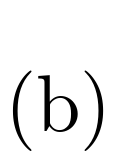
\includegraphics{figures/(b).png}

}

}

\end{minipage}%
%
\begin{minipage}[t]{0.01\linewidth}

{\centering 

~

}

\end{minipage}%
%
\begin{minipage}[t]{0.70\linewidth}

{\centering 

\raisebox{-\height}{

\includegraphics{figures/ch5/vapour_system_layout_1.png}

}

}

\end{minipage}%
%
\begin{minipage}[t]{0.15\linewidth}

{\centering 

~

}

\end{minipage}%

\caption{\label{fig-delivery-system}The three mass flow controllers
(MFCs) of the vapour delivery system are shown in (a), each with a
regulator to set the pressure at the MFC inlet. (1) is the 20 sccm
full-scale flow MFC, (2) is the 200 sccm full-scale flow MFC, and (3) is
the 500 sccm full-scale flow MFC. The device chamber, reference sensors
and other chamber peripherals are shown in (b). The components are
labelled as follows: (1) Device chamber, (2) Photoionisation detector
(PID), (3) Flowmeter from chamber to PID, (4) Micropump from chamber to
PID, (5) Relative humidity and temperature monitor.}

\end{figure}

Three mass flow controllers (MFCs) and their associated regulators sit
in a covered enclosure, seen from the front in
Figure~\ref{fig-delivery-system} (a). The MFCs are used to control the
nitrogen flow rate through two delivery lines, the carrier line and
dilution line. Each line consists of a mix of stainless steel and
flexible PVC tubing, with various Swagelok fittings and valves; these
valves include check valves, to ensure there is no vapour backflow. The
system is designed so that only one MFC delivers flow through each line.
Furthermore, the mass flow controller with a full-scale flow of 500 sccm
(standard cubic centimeters per minute) can only be directed through the
dilution line, and the mass flow controller with a full-scale flow of 20
sccm can only be directed through the carrier line. The dilution and
carrier lines merge at a mixing point about a metre before the device
chamber, which contains the device being tested. Flow through the
carrier line is bubbled through a volatile compound within a sealed 10
mL Schott bottle (Duran). A three-way valve determines whether the
analyte vapour is then carried towards the mixing point or sent to the
system exhaust.

\hypertarget{sec-reference-sensors}{%
\subsection{Reference Sensors}\label{sec-reference-sensors}}

Two reference sensors were added to the vapour delivery setup to compare
the response to vapour by the fabricated sensor device with some
reference signal. These reference sensors are a photoionisation detector
(Ametek Mocon) and a relative humidity and temperature indicator
(Telaire). The layout of these reference sensors (and their associated
peripherals) relative to the device chamber is shown in
Figure~\ref{fig-delivery-system} (b). These components are on a raised
platform directly above the mass flow controller enclosure. Vapour
flowing through the device chamber passes into a cylindrical manifold
with three outlets. One outlet is the system exhaust, one flows into
relative humidity indicator chamber, and one flows into the
photoionisation detector. A dial-controlled micro diaphragm pump is used
to set the flow rate from the manifold into the photoionisation
detector, with a flowmeter used to monitor this flow rate. The
electronic integration and programming of the relative humidity and
temperature indicator is described in Section~\ref{sec-control-system}.
The photoionisation detector was connected to a laptop directly via USB,
then controlled and monitored using the supplier-provided VOC-TRAQ II
software package.

\hypertarget{relative-humidity-and-temperature-indicator}{%
\subsubsection*{Relative Humidity and Temperature
Indicator}\label{relative-humidity-and-temperature-indicator}}
\addcontentsline{toc}{subsubsection}{Relative Humidity and Temperature
Indicator}

The relative humidity and temperature indicator used here is a
capacitive humidity sensor \autocite{Telairesensor}. It consists of a
capacitor with a hygroscopic polymer as the capacitor dielectric. As
room temperature water has a much larger dielectric constant than the
polymer dielectric, absorption of water by the polymer leads to
increased sensor capacitance \autocite{capacitivesensor}. The sensor
capacitance, corresponding to the amount of moisture absorbed by the
polymer and therefore the relative humidity, is then translated by the
sensor into a calibrated electronic output. This output is then
processed using the hardware and software described in
Section~\ref{sec-control-system} to give a value for the relative
humidity. The sensor has a quoted relative humidity (RH) accuracy of
\(\pm 2.0\)\% when RH is below 80\%, and has a quoted temperature
accuracy of 0.5°C \autocite{Telairesensor}. The absolute humidity (AH),
the mass of water vapour within a set volume, can be calculated in
gm\(^{-3}\) using Equation~\ref{eq-absolute-humidity}.
\begin{equation}\protect\hypertarget{eq-absolute-humidity}{}{
AH = C\frac{P_W}{T}
}\label{eq-absolute-humidity}\end{equation}

Here, \(C = 2.16679\) gKJ\(^{-1}\), \(P_W\) is the water vapour pressure
(in Pa) and T is the temperature (in K) \autocite{humidityformula}. For
temperatures between -20°C and 50°C, water vapour pressure \(P_W\) (in
hPa) can be approximated using Equation~\ref{eq-water-vapour-pressure}.
\begin{equation}\protect\hypertarget{eq-water-vapour-pressure}{}{
P_W = RH \times A \times 10^{(mT/(T+T_{n}))}
}\label{eq-water-vapour-pressure}\end{equation}

Here, RH is relative humidity, T is temperature in °C, \(A = 6.116441\)
hPa, \(m = 7.591386\) and \(T_{n}\) = 240.7263°C
\autocite{humidityformula}.

\hypertarget{photoionisation-detector}{%
\subsubsection*{Photoionisation
Detector}\label{photoionisation-detector}}
\addcontentsline{toc}{subsubsection}{Photoionisation Detector}

A photoionisation detector (PID) can be used to continuously monitor
volatile organic compounds by measuring the extent to which vapour
molecules passing through the detector can be ionised. A small
percentage of vapour molecules flowing into the detector diffuse into a
sensor cavity. This cavity is bounded on each side by a pair of
electrodes. A lamp in the body of the detector radiates UV light through
a window into this cavity. The vapour molecules have their outer-most
electrons excited and removed when struck with these high-energy
photons. The ionised molecules then drift towards the sensor cathode,
while free electrons drift towards the sensor anode. This results in a
current proportional to the concentration of vapour molecules in the
chamber. The current can then be amplified for a signal readout. To be
detected, the ionisation energy of the molecules being monitored cannot
exceed the energy of the incident UV light. Therefore, molecules of
clean air will not be detected. Likewise, volatile organic compounds
with high ionisation energy \(-\) such as methane \(-\) will not be
recognised by the PID. Conversely, if the energy required to ionise a
volatile of interest is relatively low, the PID will generally show a
relatively large response to that volatile
\autocite{Ionscience,PIDmanual}.

The photoionisation detector lamps used in this work each had a lamp
energy of 10.6 eV, with a quoted response time of less than 2 seconds.
Photoionisation detectors are designed to sensitively detect within a
particular concentration range. PID sensors can become less sensitive
after being exposed to very high concentrations of volatile gas. They
can also become less sensitive if exposed to high levels of humidity or
volatile substances known to contaminate the PID window, which are not
used in this thesis. The typical sensitivity range of a PID can be
stated in terms of the sensor response to isobutylene gas, which is
typically used to calibrate PID sensors. The sensitivity ranges of the
two PID sensors used here were 10 ppb \(-\) 200 ppm and 100 ppb \(-\)
2,000 ppm. Calibration with a reference gas ensures the detector reads
the true concentration of volatiles being detected, multiplied by some
previously-documented factor called a ``response factor''. However,
these response factors can vary based on the design of the PID and
various environmental factors \autocite{Ionscience,PIDmanual}.

In this work, the PID was operated without end-user calibration. PID
measurements were used to confirm the evolution of vapour presence in
the chamber over time. It should be expected that sensor sensitivity
will exhibit span drift over days or weeks, depending on changes in the
local environment, and therefore measurements should not be treated as
absolute measurements that correspond to a true concentration reading. A
sampling rate of 1 s was used for all measurements. When sampling vapour
concentration, baseline measurements of nitrogen flow through the PID
were used as the zero concentration reference point. The vapour of
interest can be delivered to the PID either through diffusion or by
means of a low-power pump. A micro diaphragm pump (Xavitech) was
selected to pump the vapour from the chamber into the PID detector. A
pump with a low maximum flow rate was selected since the PID requires an
inlet flow of less than 300 sccm. As the pump is controlled using an
unlabelled dial, a flowmeter was used to independently measure the flow
rate through the micropump into the PID.

\hypertarget{sec-control-system}{%
\subsection{Control System}\label{sec-control-system}}

The vapour delivery system was controlled and monitored from a laptop
connected to a National Instruments USB-6009 multifunction data
acquisition input/output module (DAQ). This USB-6009 DAQ connected to
the mass flow controllers and relative humidity and temperature
indicator (Telaire) via a custom-designed circuit board manufactured by
PCBway. The outputs and inputs of the USB-6009 DAQ were set using custom
LabView software. These electronic and software components of the vapour
delivery control system are described in more detail below. The
photoionisation detector (Ametek Mocon) was controlled from the same
laptop with its own prepackaged software (VOC-TRAQ II).

\hypertarget{electronics}{%
\subsubsection*{Electronics}\label{electronics}}
\addcontentsline{toc}{subsubsection}{Electronics}

\begin{figure}

\begin{minipage}[t]{0.03\linewidth}

{\centering 

\raisebox{-\height}{


\includegraphics{figures/(a).png}

}

}

\end{minipage}%
%
\begin{minipage}[t]{0.01\linewidth}

{\centering 

~

}

\end{minipage}%
%
\begin{minipage}[t]{0.45\linewidth}

{\centering 

\raisebox{-\height}{

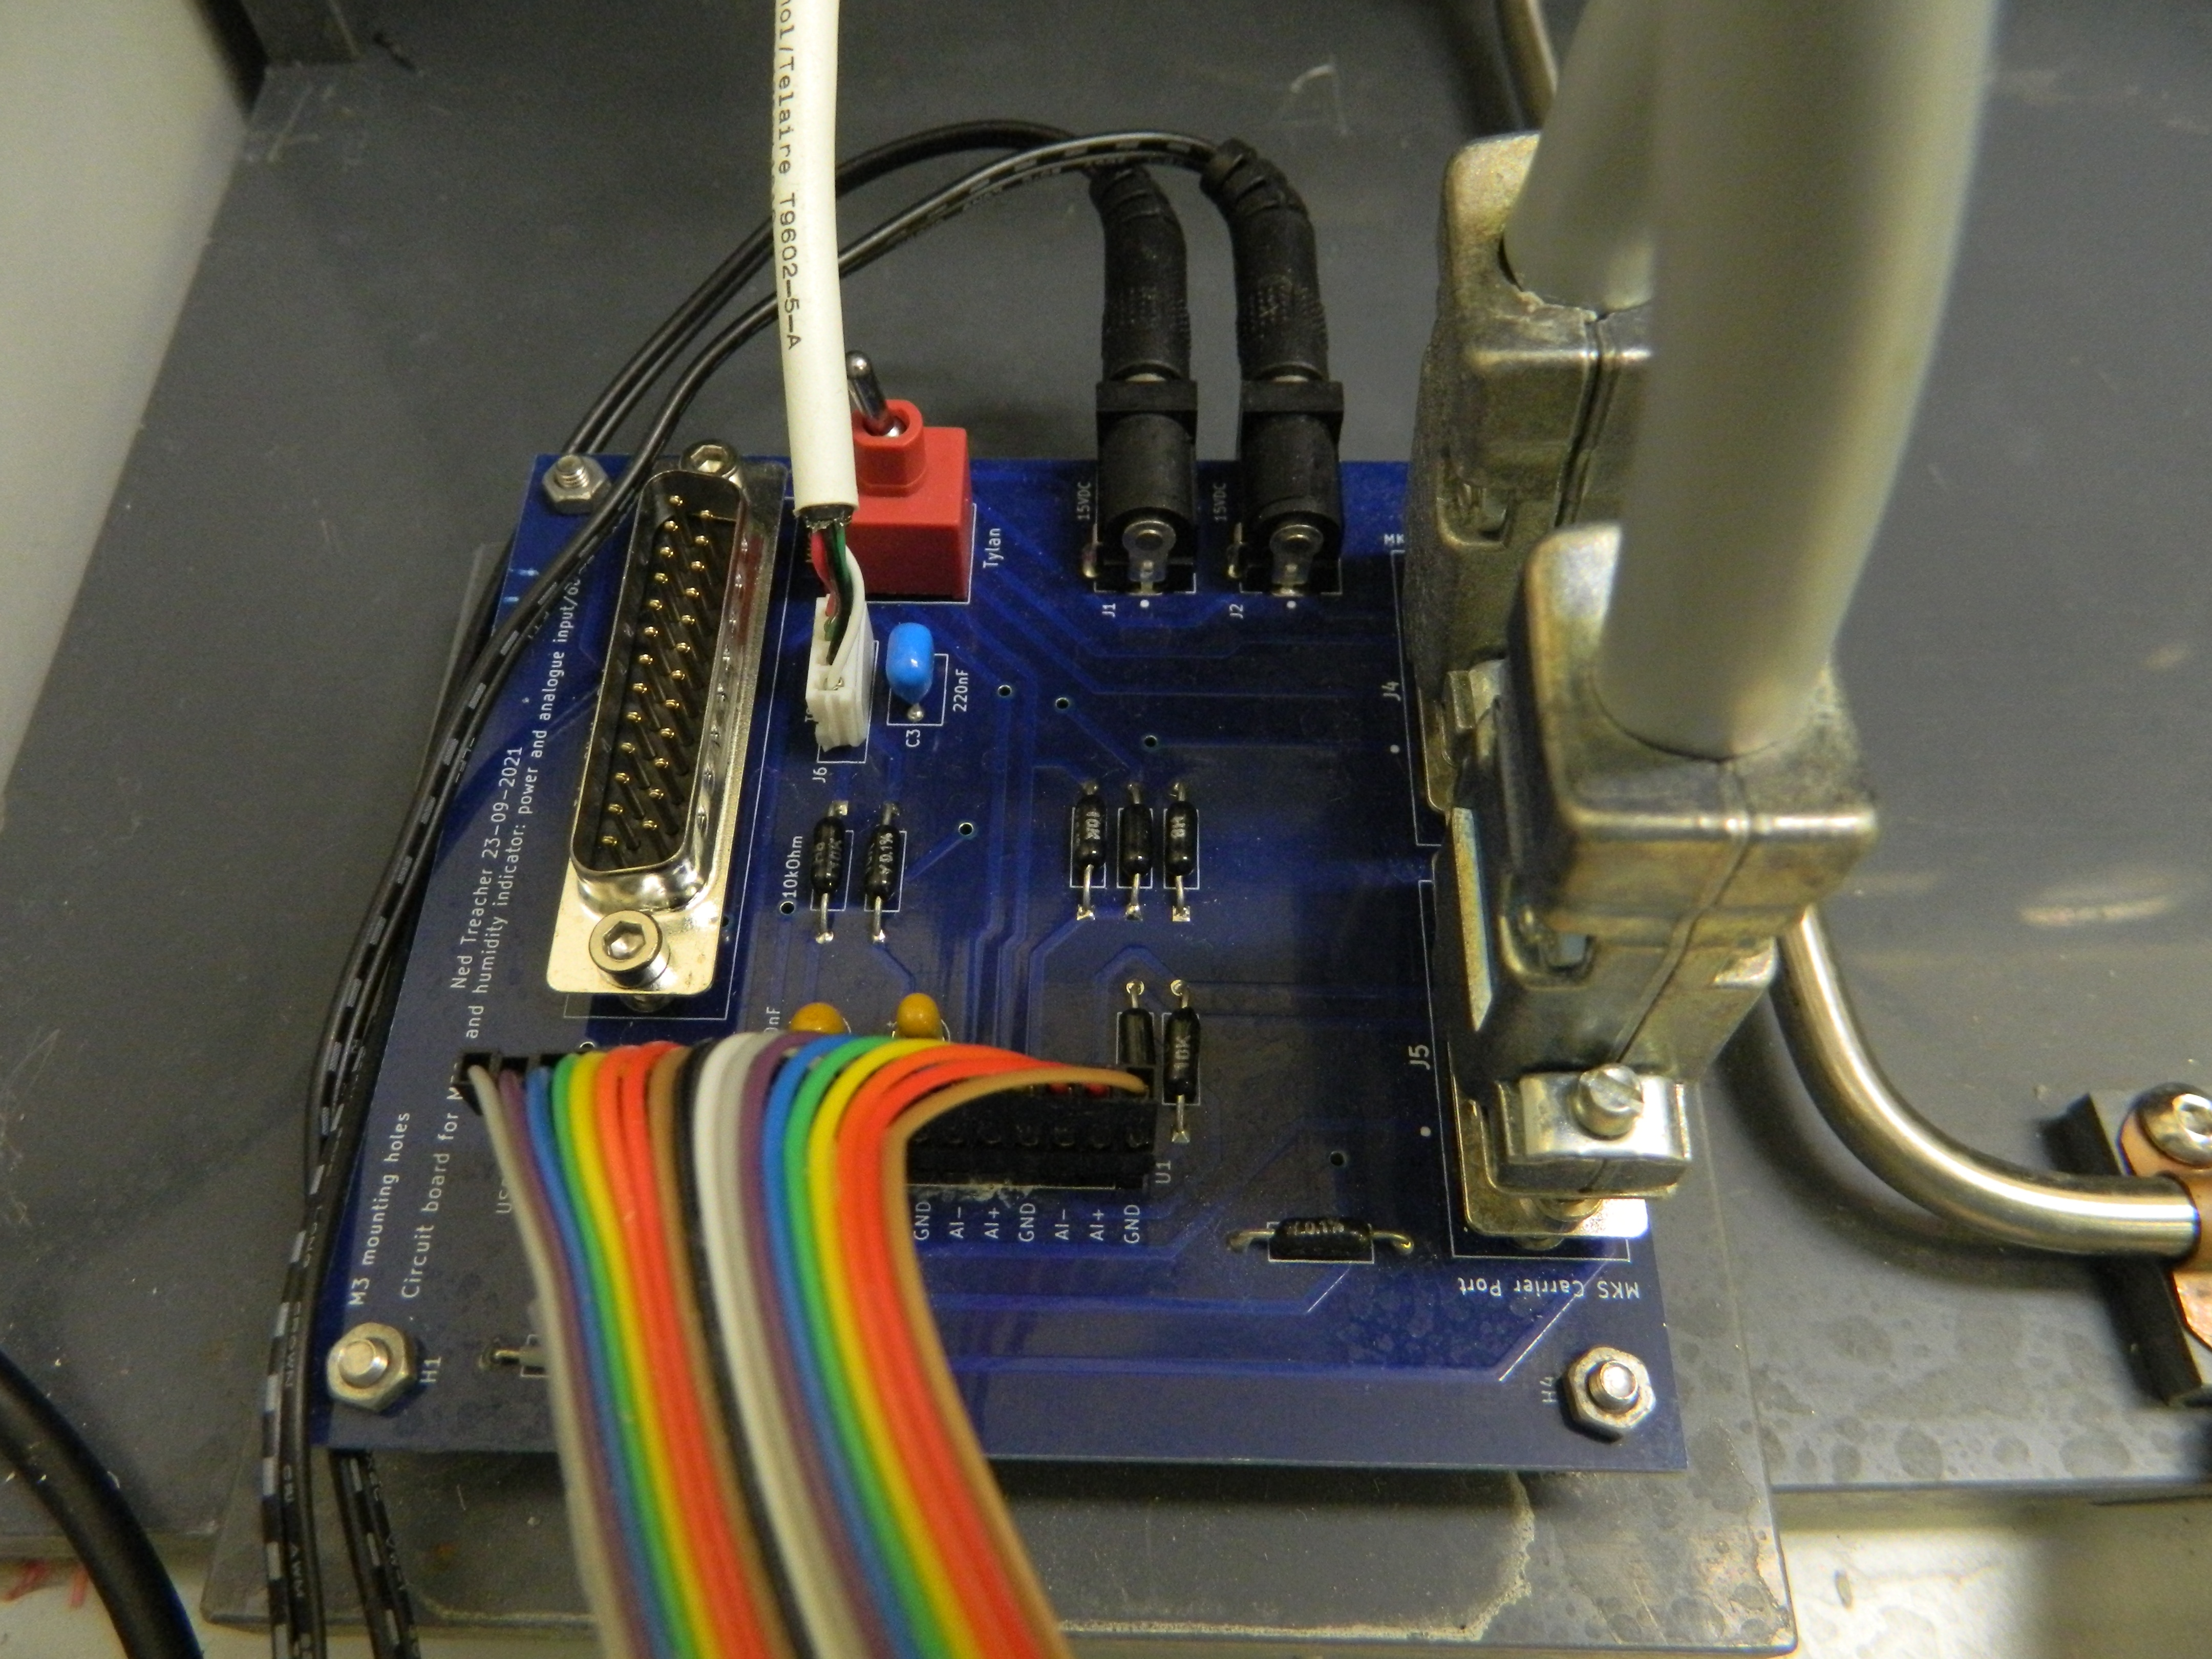
\includegraphics{figures/ch5/low_flow_config.png}

}

}

\end{minipage}%
%
\begin{minipage}[t]{0.01\linewidth}

{\centering 

~

}

\end{minipage}%
%
\begin{minipage}[t]{0.03\linewidth}

{\centering 

\raisebox{-\height}{

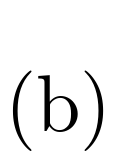
\includegraphics{figures/(b).png}

}

}

\end{minipage}%
%
\begin{minipage}[t]{0.01\linewidth}

{\centering 

~

}

\end{minipage}%
%
\begin{minipage}[t]{0.45\linewidth}

{\centering 

\raisebox{-\height}{

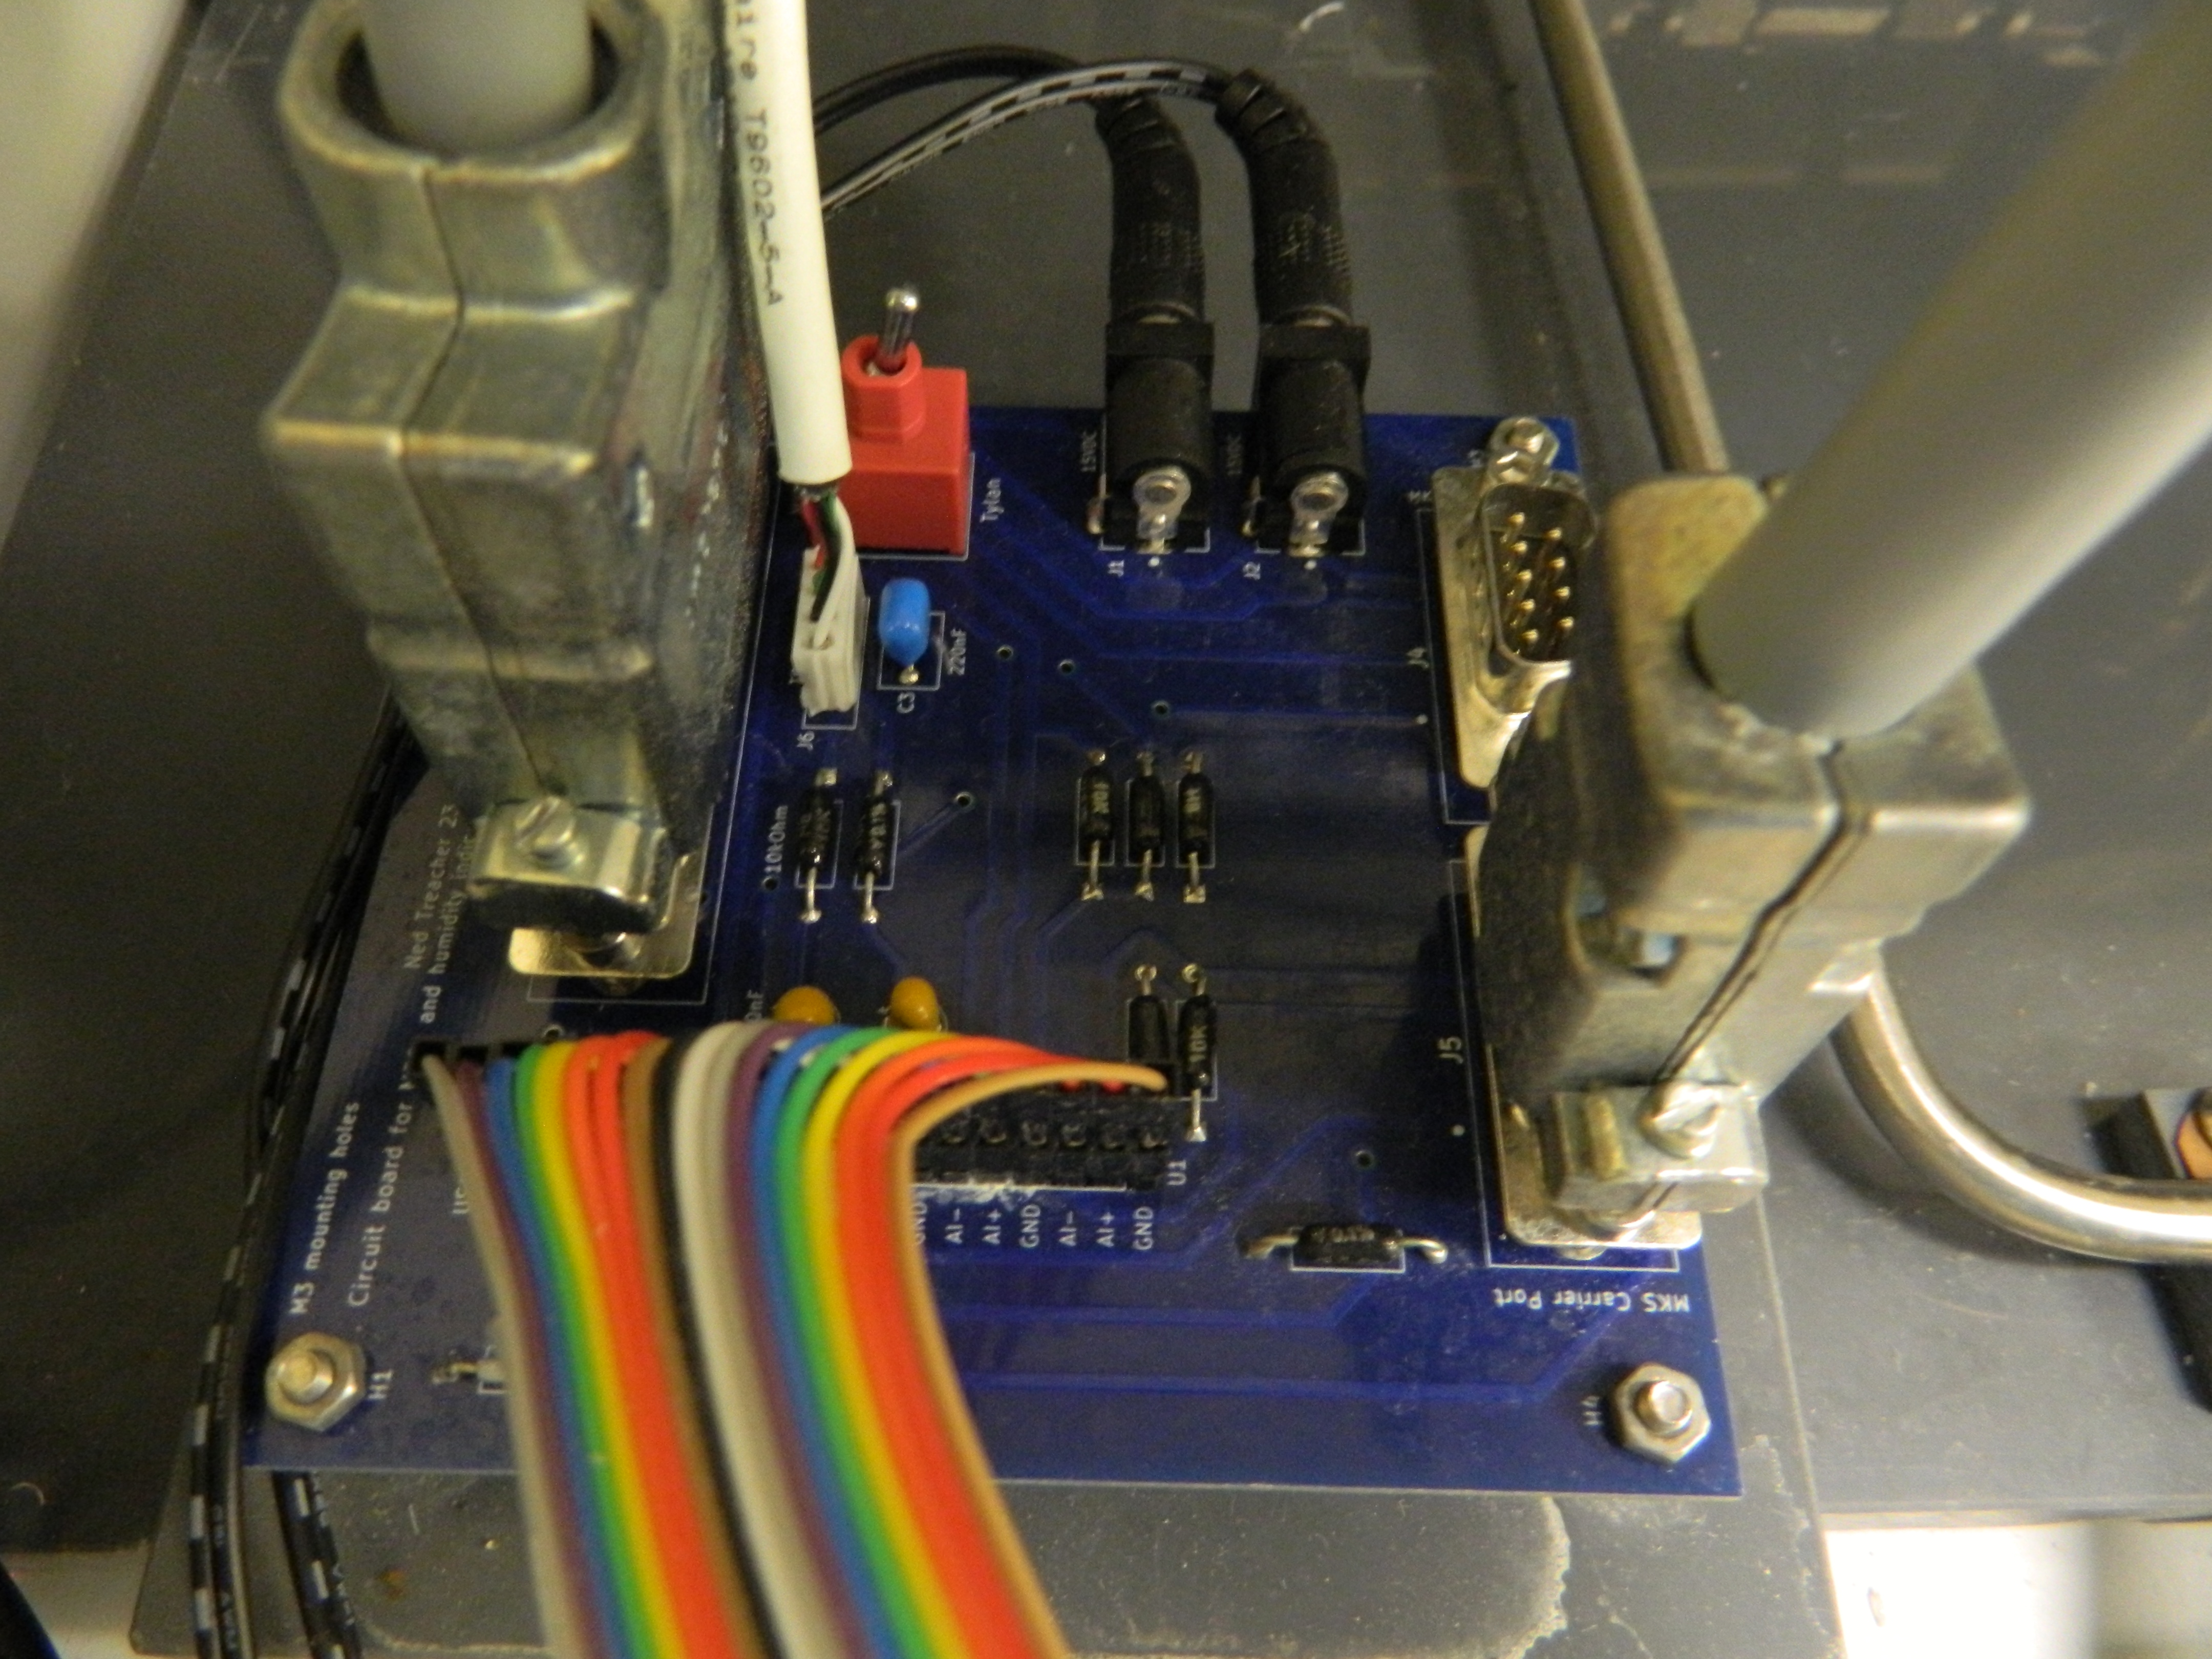
\includegraphics{figures/ch5/high_flow_config.png}

}

}

\end{minipage}%
%
\begin{minipage}[t]{0.01\linewidth}

{\centering 

~

}

\end{minipage}%

\caption{\label{fig-vapour-sensor-pcb}Images of the vapour delivery
control system circuit board, where (a) shows the low-flow configuration
and (b) shows the high-flow configuration. Components are labelled as
follows: (1) 9-pin carrier line port, (2) 9-pin dilution line port, (3)
red dilution port switch (determines which dilution line port is
active), (4) 25-pin dilution line port.}

\end{figure}

\begin{figure}

{\centering 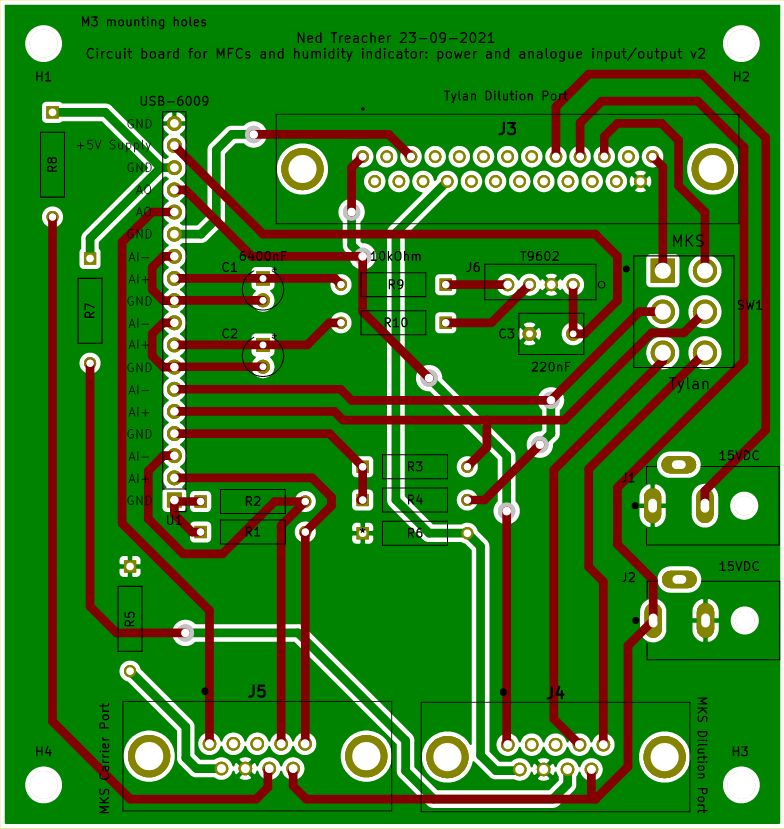
\includegraphics[width=0.95\textwidth,height=\textheight]{figures/ch5/current_PCB.png}

}

\caption{\label{fig-current-pcb-design}Circuit board schematic for
controlling and monitoring both the mass flow controllers and the
relative humidity and temperature sensor. Resistors R1-R6 are all 10
kOhm, while R7-R8 are both 0 Ohm. The circuit board was designed using
the KiCad Layout Editor.}

\end{figure}

Figure~\ref{fig-vapour-sensor-pcb} shows the control circuit board
required to connect the mass flow controllers and relative humidity
indicator to the NI USB-6009. Only one mass flow controller can be set
to provide flow to a specific line. Therefore, only two mass flow
controllers can be operational simultaneously during testing. The
control circuit board allows the user to select the two mass flow
controllers to be used during a specific test run.
Figure~\ref{fig-vapour-sensor-pcb} (a) shows the `high-flow'
configuration, where the 500 sccm full-scale MFC is connected at the
25-pin dilution line port, the 200 sccm full-scale MFC is connected to
the 9-pin carrier line port, and red dilution port switch is towards
`Tylan' (rightwards). Figure~\ref{fig-vapour-sensor-pcb} (b) shows the
`low-flow' configuration, where the 200 sccm full-scale MFC is connected
to the 9-pin dilution line port, the 20 sccm full-scale MFC is connected
to the 9-pin carrier line port and the red dilution port switch is
towards `MKS' (leftwards). The design for the circuit board is shown in
Figure~\ref{fig-current-pcb-design}, showing the USB-6009 pinout. The
relative humidity and temperature sensor is connected to the circuit
board via the T9602 footprint. In the `high-flow' configuration, the
Tylan dilution and MKS carrier ports are connected to the corresponding
MFCs, with switch SW1 is towards `Tylan'. In the `low-flow'
configuration, both MKS ports are connected, and switch SW1 is towards
`MKS'.

\hypertarget{software}{%
\subsubsection*{Software}\label{software}}
\addcontentsline{toc}{subsubsection}{Software}

Two LabView Virtual Instruments (VIs) were adapted from pre-existing VIs
for operating the mass flow controllers and monitoring vapour flow into
the device chamber, as well as monitoring temperature and humidity in
the vapour delivery system's manifold. These VIs were named
`vapour-sensor-basic.vi' and `temp-and-humidity-basic.vi'. A third VI
was developed in parallel which combined the first two Virtual
Instruments and allowed the user to set a sequence of values for the
output flow from the mass flow controllers before an experimental run.
This VI was named `vapour-sensor-sequence-timestamped.vi'. Flow rate,
relative humidity and temperature data were then saved as .lvm files.
The LabView VIs described here are available on request.

\hypertarget{sec-vapour-system-design}{%
\section{Design}\label{sec-vapour-system-design}}

\hypertarget{initial-design}{%
\subsection{Initial Design}\label{initial-design}}

\begin{figure}

{\centering 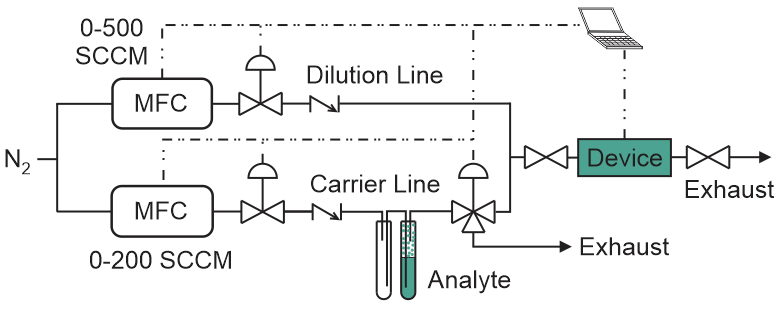
\includegraphics[width=1\textwidth,height=\textheight]{figures/ch5/PID_V0.png}

}

\caption{\label{fig-original-pid}P\&ID of the original vapour delivery
system}

\end{figure}

The initial design of the vapour delivery system, as shown in
Figure~\ref{fig-original-pid}, was relatively simple. No reference
sensors were included in the setup, and only one channel could be
characterised without opening the chamber and changing the position of
the device. However, as constructed it worked well as a self-contained
system, which was able to deliver vapour to a device channel while
measuring current across the channel. A 500 sccm full-range MFC (Tylan)
was placed on the dilution line, and a 200 sccm full-range MFC (Tylan)
was placed on the carrier line. A glass container for analyte was
present on the carrier line, with a vapour trap upstream to collect any
backflow. The vapour trap was removed in later iterations due to the
presence of a check valve to prevent backflow. The device chamber and
mass flow controllers were connected to a laptop and an Agilent 4156C
semiconductor parameter analyser and controlled using LabView.

\hypertarget{sec-vapour-system-design-1}{%
\subsection{Stage I Design}\label{sec-vapour-system-design-1}}

\begin{figure}

{\centering 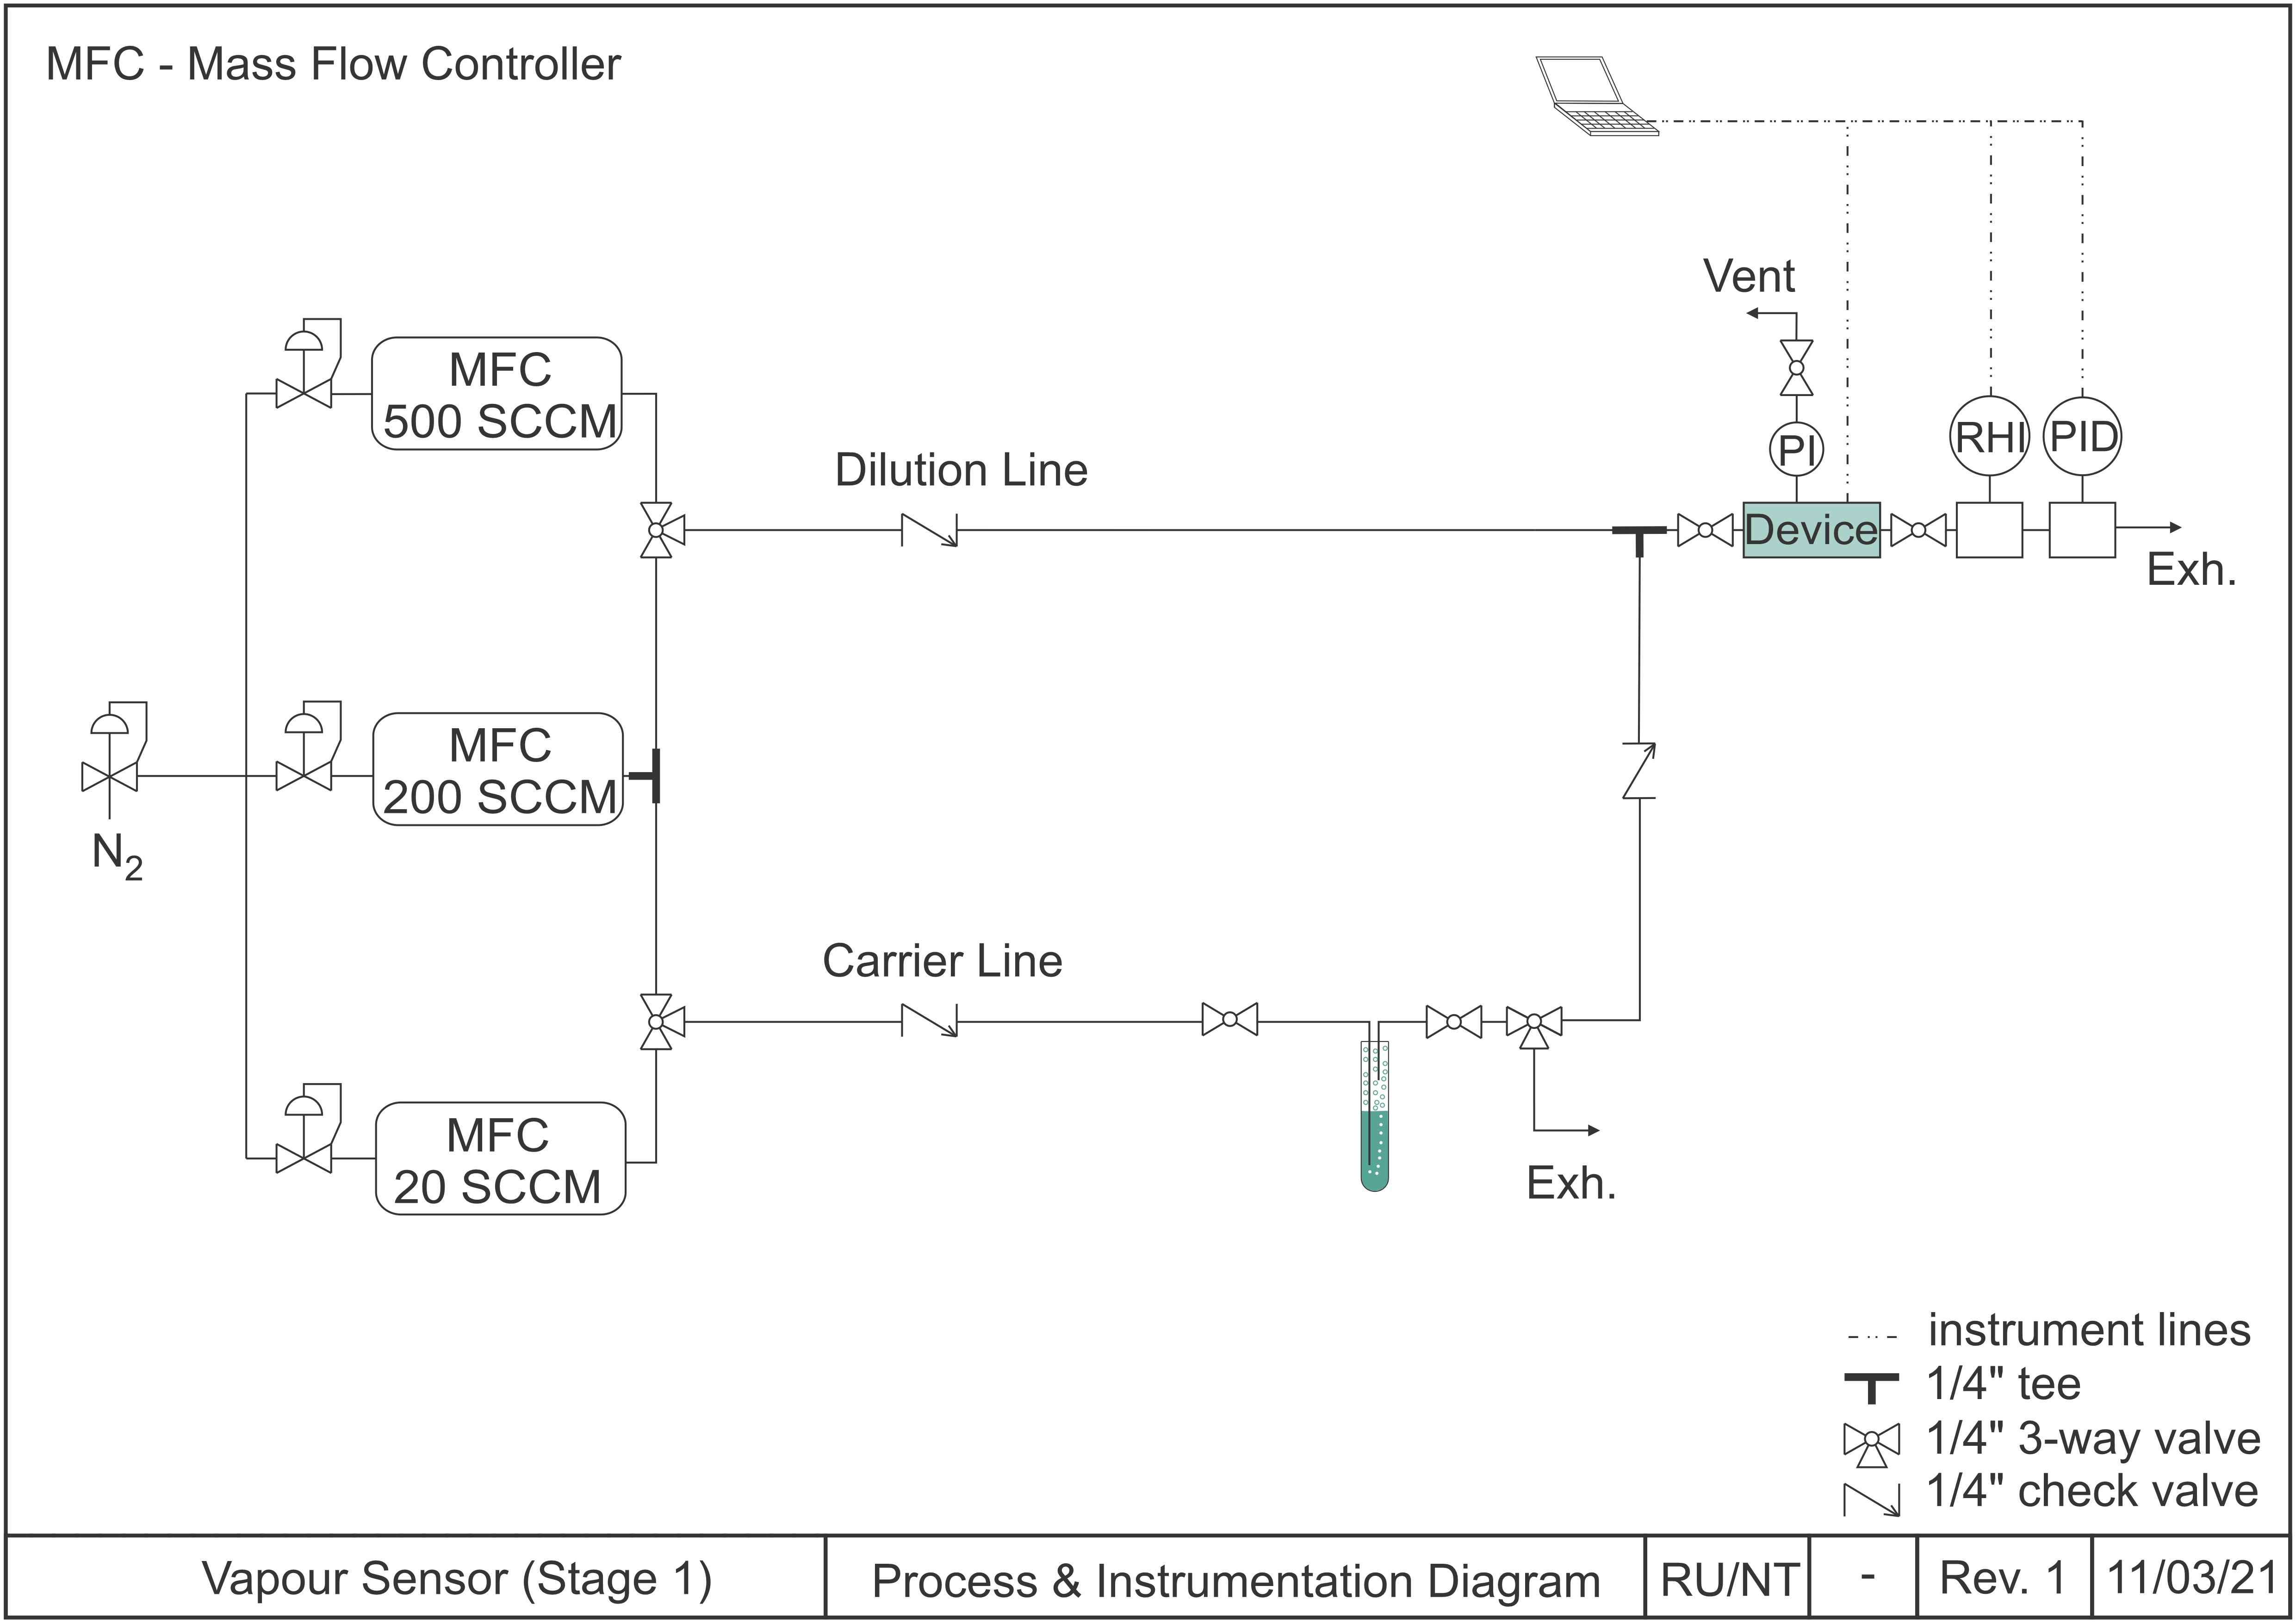
\includegraphics[width=1\textwidth,height=\textheight]{figures/ch5/PID_V1.png}

}

\caption{\label{fig-stage-1-pid}P\&ID of the Stage I vapour delivery
system.}

\end{figure}

The first stage of the vapour delivery system redesign, as shown in
Figure~\ref{fig-stage-1-pid}, was implemented in Nov 2021. This system
introduced the ability to use a 20 sccm full-range MFC (MKS Instruments)
for carrier line flow and a 200 sccm full-range MFC (MKS Instruments)
for either carrier or dilution line flow, to give better control when
using low flow rates. The reference sensors were also implemented, with
each sensor connected in parallel to the chamber exhaust. Through
testing the system with ethanol and acetone as analytes, the following
issues with this implementation of the setup were identified:

\begin{itemize}
\item
  With the system connected to the lab supply of nitrogen, pressure
  changes in the line due to nitrogen use elsewhere in the lab impacted
  the pressure at the MFCs and the flow through the lines.
\item
  The pressure indicator used for the device chamber had a much wider
  range than the pressure reached before nitrogen began to leak out of
  the PVC tubing; this meant pressure changes in the chamber, resulting
  from closing the exit valves while nitrogen flow entered the chamber,
  did not register on the indicator.
\item
  The PID responded unexpectedly slowly to changes in vapour
  concentration in the chamber. For example, after acetone or ethanol
  vapour had been run through the chamber, running clean nitrogen
  through the system for 3 hours was required before the PID returned to
  a constant baseline reading.
\item
  There was no way to ensure the device chamber was free of analyte
  vapour before an experimental run aside from running nitrogen through
  the dilution line. After prolonged use, condensed analyte was
  sometimes visible in the PVC lines of the delivery system.
\end{itemize}

These issues, along with various minor structural and design issues,
were addressed in the second-stage implementation of the system.

\hypertarget{stage-ii-design}{%
\subsection{Stage II Design}\label{stage-ii-design}}

\begin{figure}

{\centering 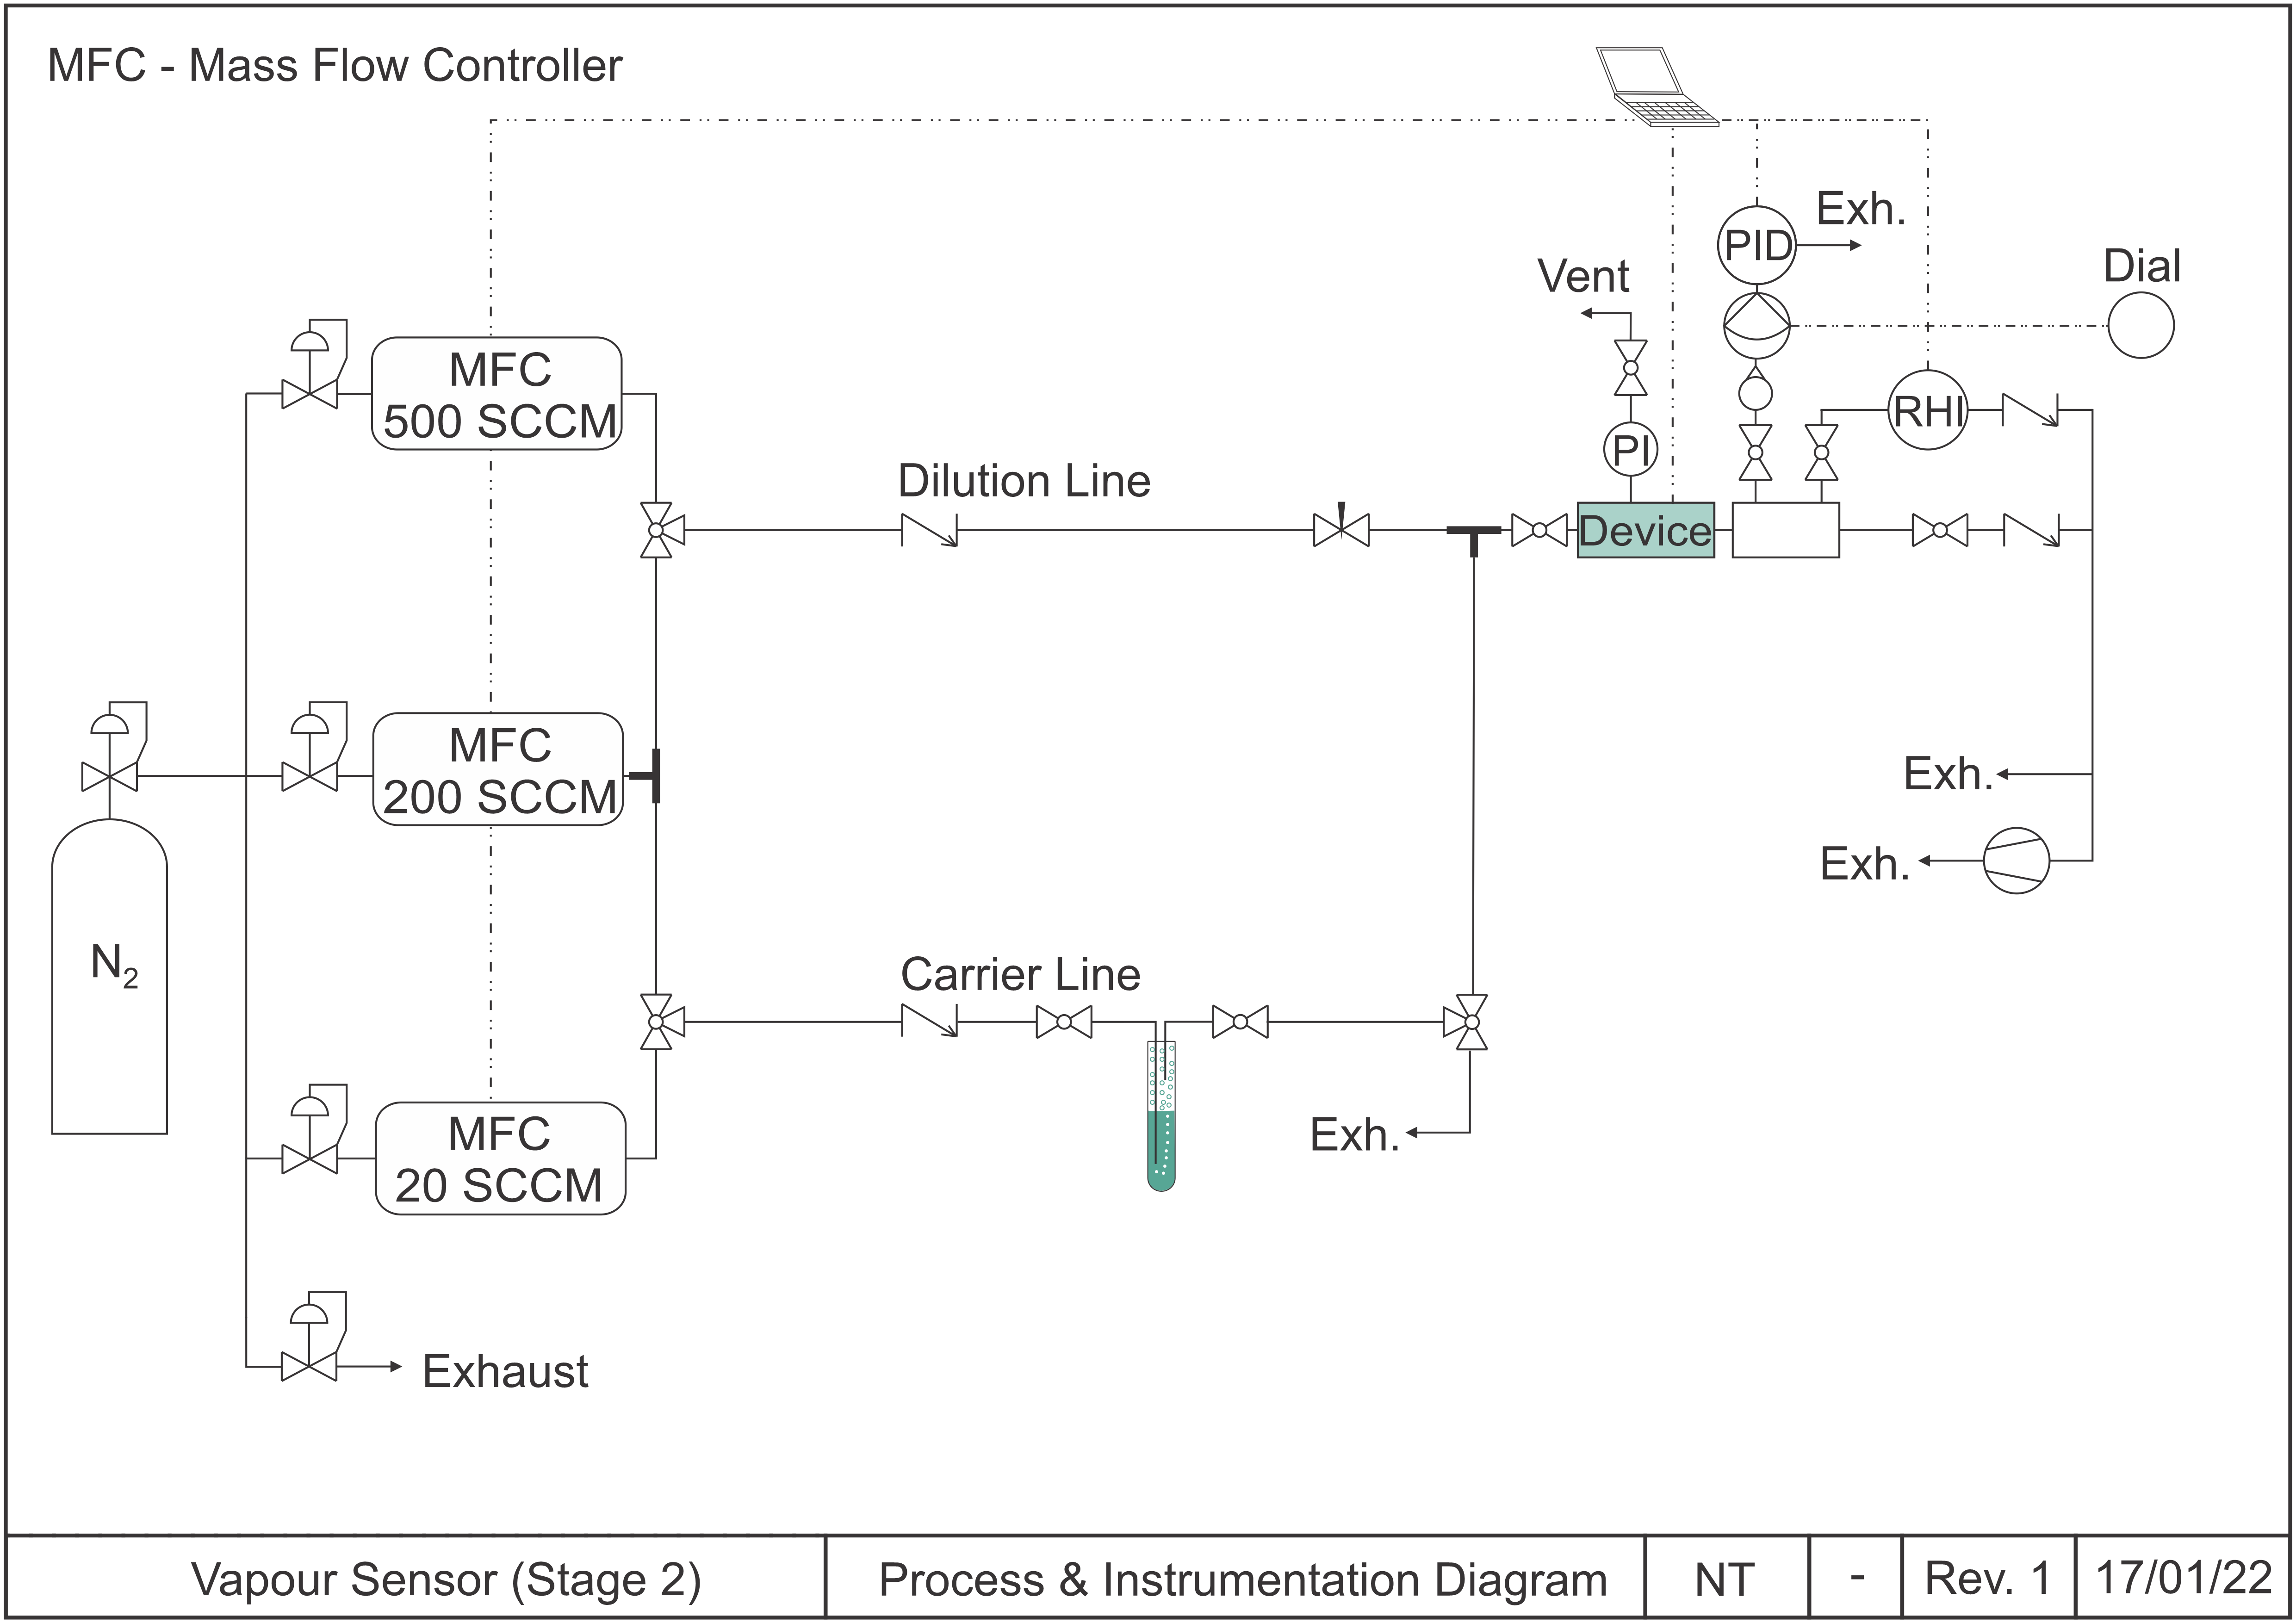
\includegraphics[width=1\textwidth,height=\textheight]{figures/ch5/PID_V2.png}

}

\caption{\label{fig-stage-2-pid}Process \& instrumentation diagram
(P\&ID) of the second-stage design for the vapour delivery system. Red
outlines indicate additions introduced to the system subsequent to the
first stage design.}

\end{figure}

Figure~\ref{fig-stage-2-pid} gives an overview of the second-stage
design for the vapour delivery system setup. This stage of the redesign
was implemented between Jan and May 2022. Changes from the first stage
included:

\begin{itemize}
\item
  The addition of a N\(_2\) cylinder (152D size) as the source of
  nitrogen for the system to replace the lab supply.
\item
  A pressure indicator with a lower pressure range was used, which could
  register pressure changes within the device chamber.
\item
  A chamber manifold was placed before the exhaust with outlets into the
  PID and RHI.
\item
  A micro diaphragm pump was introduced between the manifold and PID to
  supply the PID with vapour from the chamber, and a flowmeter was
  placed before the pump to measure the flow rate out of the chamber to
  the PID. The PID was then seen to respond quickly to system changes
  (discussed further in Section~\ref{sec-calibration}).
\item
  A piece of PVC tubing was placed at the PID outlet to limit air from
  the fumehood entering the PID when the micropump was off.
\item
  Valves were placed before all system components so that the device
  chamber and post-analyte bottle carrier line could be evacuated with a
  roughing pump without potentially affecting components.
\item
  Check valves were placed at the exhaust to prevent backflow from the
  roughing pump into the delivery system.
\end{itemize}

These changes largely addressed the issues identified in
Section~\ref{sec-vapour-system-design-1}.

\hypertarget{sec-calibration}{%
\section{Calibration and Measurements of Vapour
Flow}\label{sec-calibration}}

\hypertarget{sec-flow-calibration}{%
\subsection{Chamber Flow Calibration}\label{sec-flow-calibration}}

\begin{figure}

{\centering 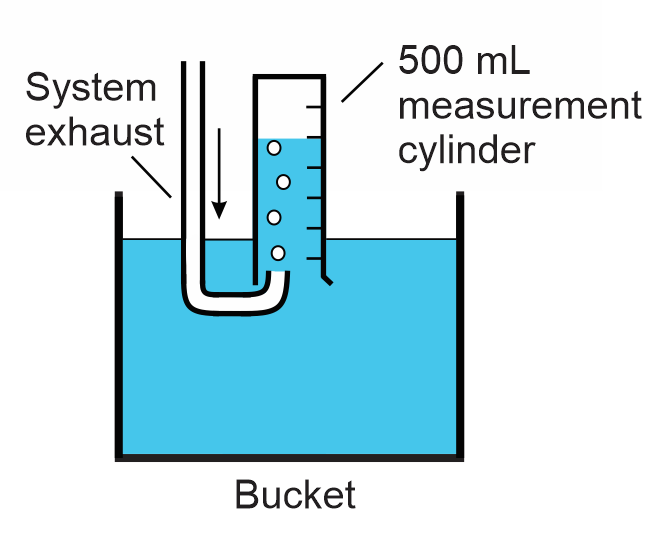
\includegraphics[width=0.45\textwidth,height=\textheight]{figures/ch5/water_displacement.png}

}

\caption{\label{fig-water-displacement}Setup for calibration of mass
flow controllers using the water displacement method.}

\end{figure}

A water displacement test was carried out to determine the relationship
between the flow rate measured by the mass flow controllers and the
actual flow rate passing through the chamber. All valves were set so
that both the dilution and carrier lines followed a single path. Both
these paths went through the device chamber and out through the system
exhaust. An empty analyte bottle was placed on the carrier line. The
system exhaust was placed into a bucket filled with tap water, with the
outlet sitting beneath an upturned 500 mL measurement cylinder, as
pictured in Figure~\ref{fig-water-displacement}. The cylinder was used
to measure the volume of displaced water over time, which is equivalent
to the rate of change of nitrogen volume entering the cylinder from the
exhaust. Measurements were taken from the bottom of the meniscus of the
water in the cylinder. As leaks from the manifold, chamber and exhaust
line were not detected when leak testing with bubble solution, it can be
safely assumed that the rate at which nitrogen exits the exhaust is
equivalent to the nitrogen flow rate through the device chamber.

\begin{figure}

\begin{minipage}[t]{0.03\linewidth}

{\centering 

\raisebox{-\height}{


\includegraphics{figures/(a).png}

}

}

\end{minipage}%
%
\begin{minipage}[t]{0.01\linewidth}

{\centering 

~

}

\end{minipage}%
%
\begin{minipage}[t]{0.45\linewidth}

{\centering 

\raisebox{-\height}{

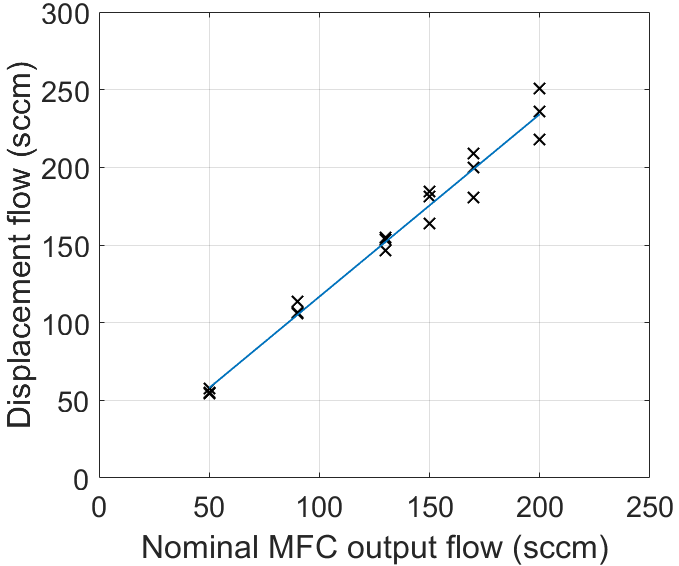
\includegraphics{figures/ch5/200sccmMFC_carrierline_thruchamber.png}

}

}

\end{minipage}%
%
\begin{minipage}[t]{0.01\linewidth}

{\centering 

~

}

\end{minipage}%
%
\begin{minipage}[t]{0.03\linewidth}

{\centering 

\raisebox{-\height}{

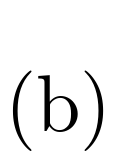
\includegraphics{figures/(b).png}

}

}

\end{minipage}%
%
\begin{minipage}[t]{0.01\linewidth}

{\centering 

~

}

\end{minipage}%
%
\begin{minipage}[t]{0.45\linewidth}

{\centering 

\raisebox{-\height}{

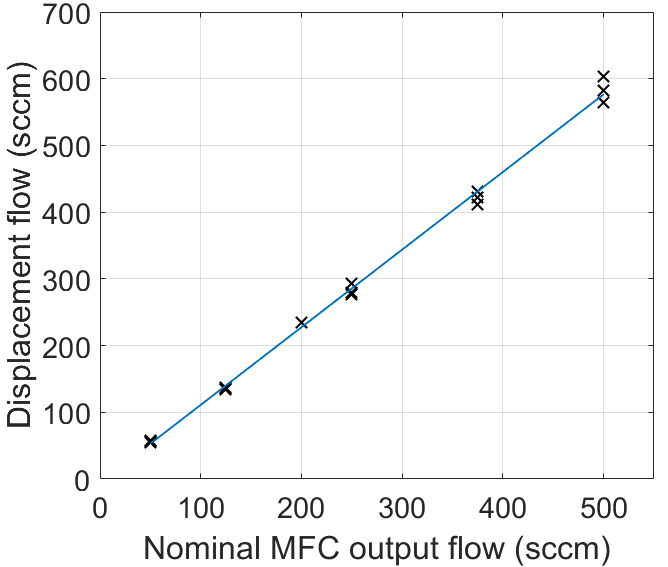
\includegraphics{figures/ch5/500sccmMFC_dilutionline_thruchamber.png}

}

}

\end{minipage}%
%
\begin{minipage}[t]{0.01\linewidth}

{\centering 

~

}

\end{minipage}%

\caption{\label{fig-MFC-calibration-curves}The nominal flow rate as
measured by the mass flow controller compared to the actual flow rate
measured using water displacement testing, shown for the 200 sccm
full-scale mas flow controller placed through the carrier line in (a),
and for the 500 sccm full-scale mass flow controller placed through the
dilution line in (b). Three water displacement tests were performed for
each constant flow rate.}

\end{figure}

The time taken to displace 50 mL of water was measured three times for a
series of constant flow rates, both for the 200 sccm MFC (MKS) on the
carrier line and the 500 sccm MFC (Tylan) on the dilution line. The
displacement flow rate corresponding to each measurement could then be
found by dividing volume by time. These measurements, of displacement
flow relative to nominal flow through the MFC, are shown in
Figure~\ref{fig-MFC-calibration-curves} (a) and (b) respectively. The
increased uncertainty for higher flow measurements is largely due to
rapid flows being more difficult to measure precisely. However,
increased instability of flow at higher flow rates may also contribute.
A strong linear relationship between the nominal flow reading and actual
flow was identified. A linear least-squares fit with 95\% confidence
interval was performed, where coefficients \(a_1\) and \(a_2\) were
found for the linear relationship \(D = a_1d + a_2\). Here, \(d\) is
nominal flow from the MFC and \(D\) is measured displacement flow. For
the 200 sccm MFC flow through the carrier line, values of
\(a_1 = 1.18\pm0.09\) and \(a_2 = -1\pm13\) were obtained, while for the
500 sccm MFC flow through the dilution line, values of
\(a_1 = 1.16\pm0.04\) and \(a_2 = -5\pm10\) were obtained.

It appears that the offset between the measured displacement flow and
nominal output flow is not due to leaks in the system, since the offset
indicates measured flow exceeds the nominal flow. Instead, the offset
appears to be a systematic error introduced by the electronics or
software used to record the output flow from the MFCs. The identical
offset between measured and nominal flow observed for each MFC, even
when placed on different lines to the chamber, further strengthens the
likelihood of the offset being due to the control side of the system.
Furthermore, as both the carrier and dilution MFCs show readings with
the same offset multiplier within a 95\% confidence interval, the same
offset should apply to a mixture of flows on each line. For example, a
200 sccm nominal flow through the dilution line from the 500 sccm
full-scale MFC should have a roughly identical actual flow rate to a 50
sccm nominal flow through the dilution line and a 150 sccm flow through
the carrier line. In this work, tests performed with the vapour delivery
system have flow rate stated in terms of their nominal value. However,
the reader should keep in mind the \(1.16-1.18 \times\) offset between
the nominal and actual chamber flow.

\begin{figure}

{\centering 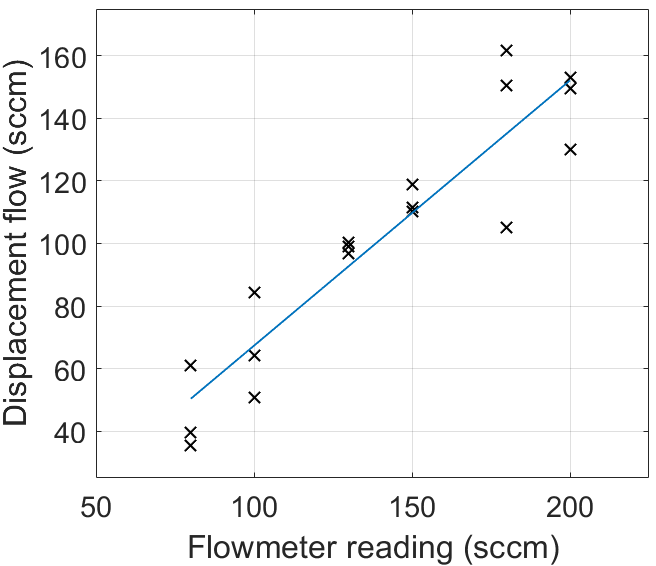
\includegraphics[width=0.45\textwidth,height=\textheight]{figures/ch5/PID_flowmeter.png}

}

\caption{\label{fig-flowmeter-calibration}Comparison of flowmeter
readings with flow measurements from water displacement testing. Three
water displacement tests were performed for each constant flow rate.}

\end{figure}

The time taken to displace a fixed water volume was also measured three
times for a series of constant flow rates through the flowmeter from the
chamber to exhaust. A least-squares linear relationship was obtained
between flowmeter readings and actual displacement, as shown in
Figure~\ref{fig-flowmeter-calibration}. Expressing the relationship as
\(D = b_1f + b_2\), where \(f\) is the flowmeter reading and \(D\) is
measured displacement flow, values of \(b_1 = 0.85\pm0.2\) and
\(b_2 = -18\pm26\) were obtained. The flow as read from the flowmeter
became less stable for flows above 150 sccm and below 130 sccm,
increasing measurement uncertainty. To understand the cause of this
instability, flow through the chamber was placed directly through the
flowmeter without the micropump present. Relatively stable measurements
could then be achieved, indicating that the flow rate instability
results from the micropump used for vapour delivery when used outside
the 130 \(-\) 150 sccm range. The micropump flow measured as 150 sccm on
the flowmeter was generally used when measuring vapour flow through the
delivery system to the photoionisation detector.
Figure~\ref{fig-flowmeter-calibration} indicates 150 sccm on the
flowmeter corresponds to \(\sim\) 110 sccm of actual flow.

\hypertarget{sec-responses-to-vapour}{%
\subsection{Sensor Responses to Vapour
Flow}\label{sec-responses-to-vapour}}

\begin{figure}

{\centering 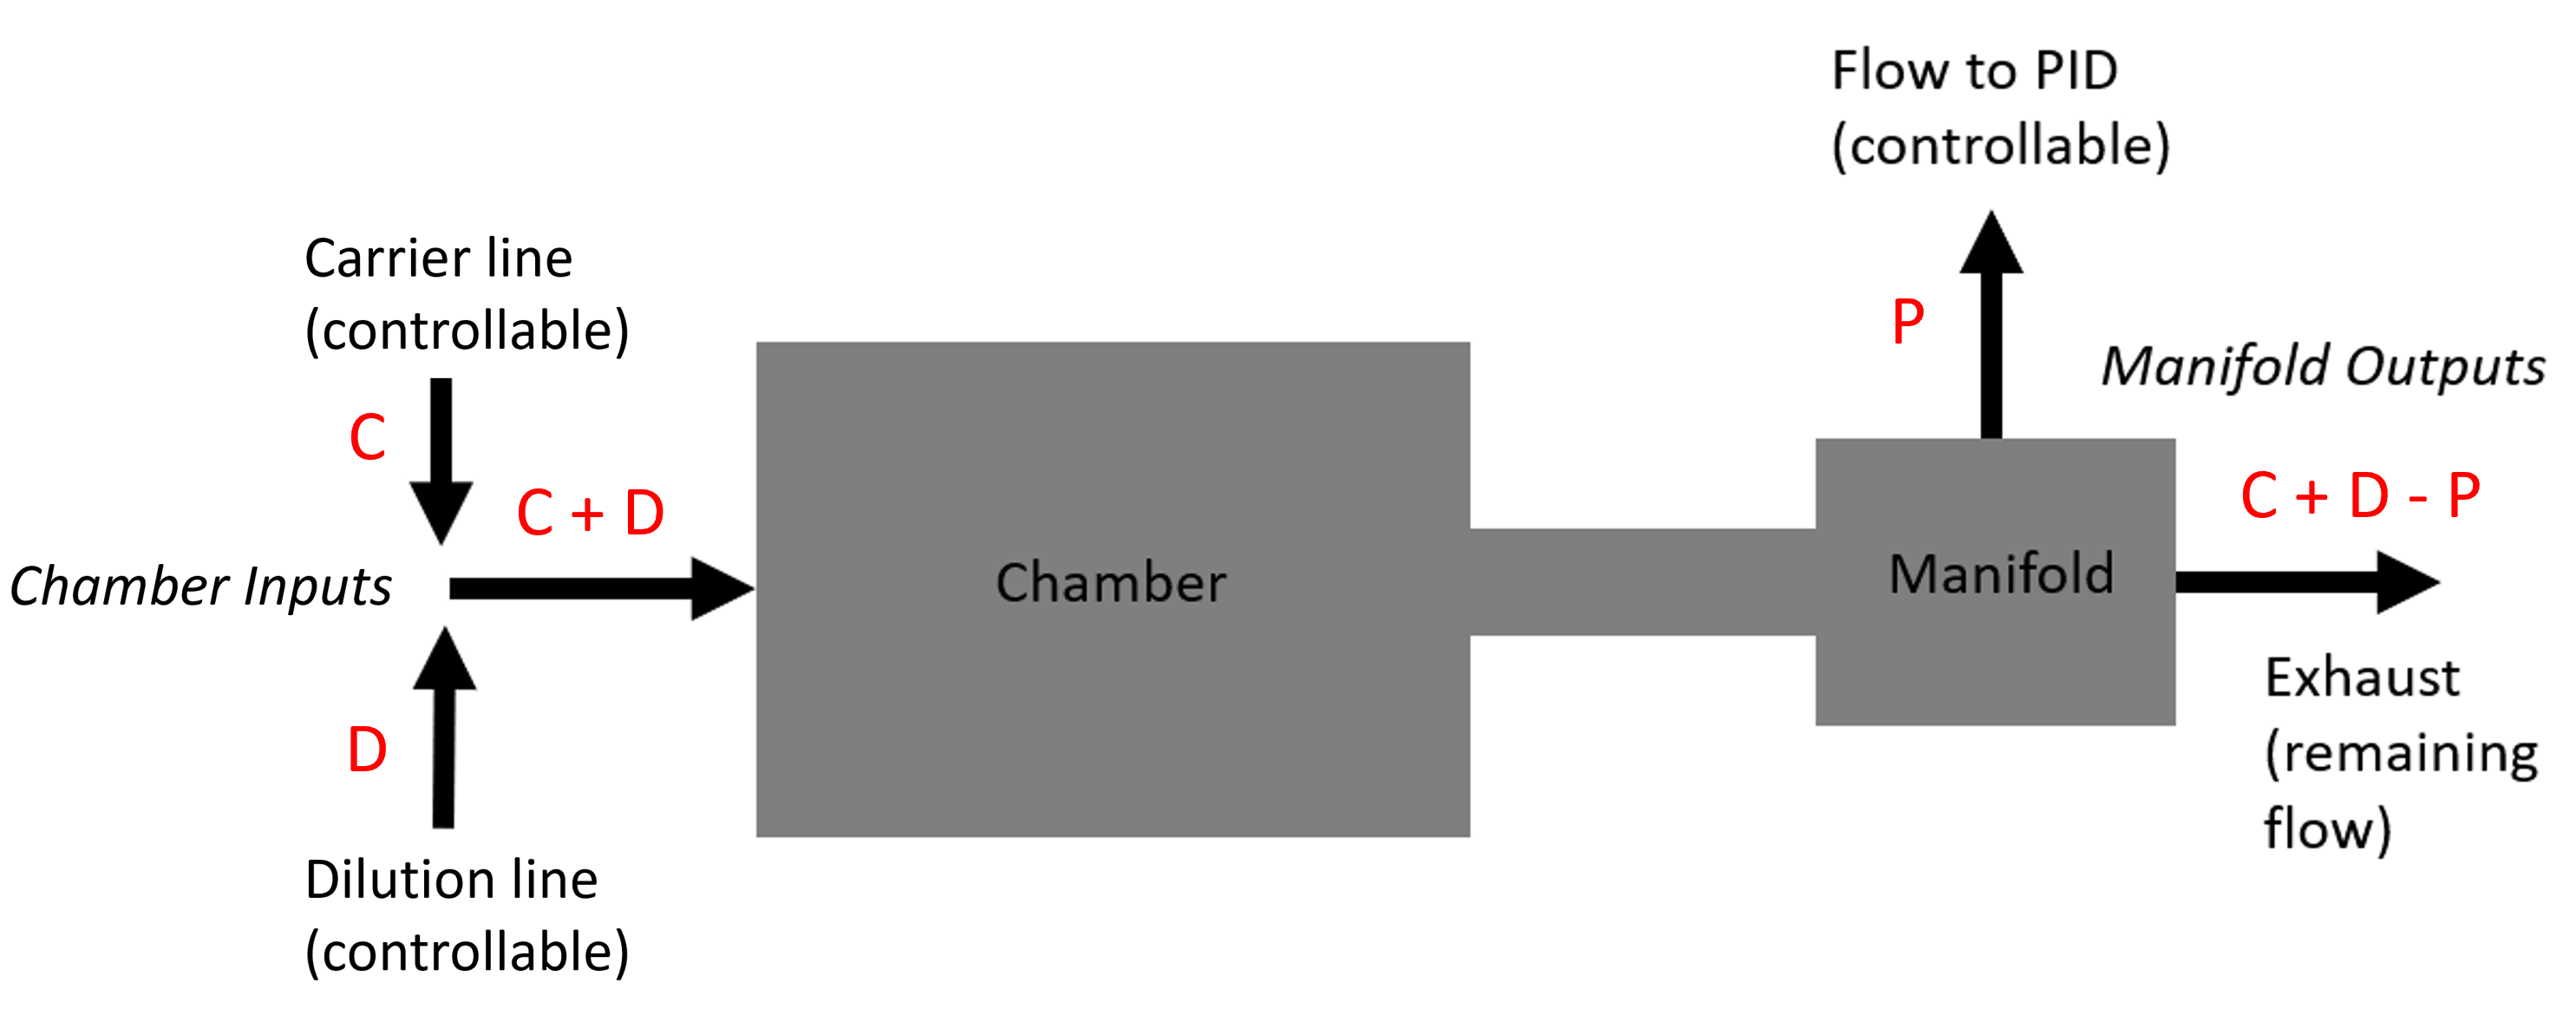
\includegraphics[width=1\textwidth,height=\textheight]{figures/ch5/chamber-manifold-v2.png}

}

\caption{\label{fig-chamber-schematic}Simplified schematic showing the
flow into and out of the device chamber and manifold of the delivery
system. The input flows from the carrier and dilution line are
represented by C and D, and the output flow through the PID is
represented by P. The exhaust can either flow past the relative humidity
indicator or straight to the fumehood. This diagram assumes that flow
through leaks in the chamber and manifold is low enough to be considered
negligible, which was confirmed by leak testing with bubble solution.}

\end{figure}

Once the rate of flow through the device chamber had been calibrated,
the correct operation of the reference sensors used in the system was
verified. Various flow rates in and out of the chamber were used to
calibrate and verify the reference sensors. These flows in and out of
the chamber are labelled on the simplified schematic in
Figure~\ref{fig-chamber-schematic}. Note that the labels on this
schematic assume that nitrogen compression at any point within this
schematic is negligible. Section~\ref{sec-flow-calibration} shows that a
200 sccm flow into the chamber corresponds to an actual rate for C + D
of \(\sim\) 230 sccm. If a 150 sccm flow rate as measured by the
flowmeter is pumped out through the PID,
Section~\ref{sec-flow-calibration} shows that P \(\sim\) 110 sccm. This
means that \(\sim\) 50\% of the flow through the chamber exits via the
PID. If a 100 sccm flowmeter rate is pumped through the PID, P \(\sim\)
70 sccm, and therefore \(\sim\) 30\% of the chamber flow exits through
the PID.

\hypertarget{relative-humidity-indicator}{%
\subsubsection*{Relative Humidity
Indicator}\label{relative-humidity-indicator}}
\addcontentsline{toc}{subsubsection}{Relative Humidity Indicator}

To test the relative humidity indicator (RHI), all valves out of the
chamber were sealed except for the valve for the relative humidity
indicator chamber. This meant all flow coming out of the system would
pass through the relative humidity indicator chamber (P = 0 sccm and
exhaust goes to RHI in Figure~\ref{fig-chamber-schematic}). Continuous
nitrogen flow was then placed through the chamber until relative
humidity dropped to about 20\%. 10 mL of deionised water was placed into
the analyte bottle. A series of different flow rates through each line
was sent to the chamber, with the sequence of flow rates shown in
Table~\ref{tbl-RHI-flow-sequence} (t = time, C = carrier line flow rate,
D = dilution line flow rate). Note that between 200 s and 600 s, the
total flow rate remains the same, but the ratio of dilution to carrier
flow differs.

\hypertarget{tbl-RHI-flow-sequence}{}
\begin{longtable}[]{@{}lll@{}}
\caption{\label{tbl-RHI-flow-sequence}Flow sequence for testing relative
humidity indicator.}\tabularnewline
\toprule\noalign{}
t (s) & C (sccm) & D (sccm) \\
\midrule\noalign{}
\endfirsthead
\toprule\noalign{}
t (s) & C (sccm) & D (sccm) \\
\midrule\noalign{}
\endhead
\bottomrule\noalign{}
\endlastfoot
200 & 0 & 400 \\
200 & 100 & 300 \\
200 & 200 & 200 \\
200 & 200 & 100 \\
200 & 200 & 0 \\
\end{longtable}

\begin{figure}

{\centering 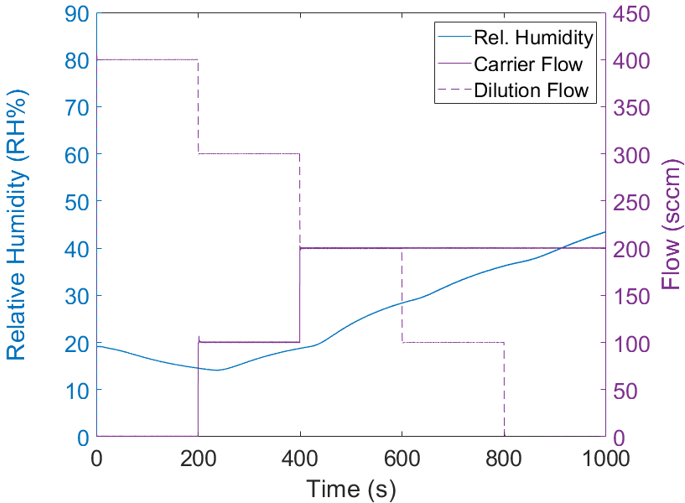
\includegraphics[width=0.65\textwidth,height=\textheight]{figures/ch5/RHI_verification.png}

}

\caption{\label{fig-RHI-verification}Relative humidity readouts from the
relative humidity indicator juxtaposed with flow rates from the dilution
line and carrier lines of the vapour system, with 10 mL deionised water
in the carrier line analyte bottle.}

\end{figure}

Figure~\ref{fig-RHI-verification} shows that the Telaire sensor records
decreased humidity after flow exclusively from the dilution line and
increased humidity after flow from the analyte bottle. It also shows
that in regular 200 s intervals, the rate of relative humidity change
increases and then begins to stabilise. Each accelerated change in
relative humidity occurs about 50 s after a corresponding increase in
flow through the carrier line. It appears a 50 s period passes before an
increased concentration of water vapour due to increased carrier flow
first reaches the relative humidity indicator. Over the full 800 s of
carrier line flow, relative humidity increases from a minimum of
\(14.0\pm2.0\)\% to a maximum of \(43.6\pm2.0\)\%. The temperature in
the chamber remained between 21.0\pm0.5°C and 22.0\pm0.5°C over the
entire measurement period. Combining equations
Equation~\ref{eq-absolute-humidity} and
Equation~\ref{eq-water-vapour-pressure} from
Section~\ref{sec-reference-sensors}, we find that the absolute humidity
in the chamber reaches a low of \(2.6\pm0.4\) gm\(^{-3}\) at 238.1 s,
38.1 s after the initial onset of carrier flow, and a high of
\(8.4\pm0.5\) gm\(^{-3}\) at 998.8 s, after 798.8 s of carrier flow
through the chamber. The clear response of the Telaire RHI to increased
water vapour flow confirms that this sensor is working.

\hypertarget{photoionisation-detector-with-continuous-vapour-flow}{%
\subsubsection*{Photoionisation Detector with Continuous Vapour
Flow}\label{photoionisation-detector-with-continuous-vapour-flow}}
\addcontentsline{toc}{subsubsection}{Photoionisation Detector with
Continuous Vapour Flow}

To test the photoionisation detector, the device chamber and carrier
line were first purged of vapour through the exhaust using a roughing
pump, with the PID valve closed to protect it from the pump. The PID
valve was then opened, the micropump was set to 150 sccm as read by the
flowmeter. During testing with the PID, the total flow into the chamber
was set at 200 sccm as read by the Tylan mass flow controllers. The
calibration curves in Section~\ref{sec-flow-calibration} show that the
actual flow C + D was then therefore approximately the same as the
actual flow rate into the PID, P. A flow of 200 sccm nitrogen was placed
through the dilution line to the chamber for 10 minutes until successive
concentration readings from the PID were either approximately constant,
or until baseline drift was small enough to be considered negligible.
These measurements were then used as the baseline (0 ppm) for subsequent
measurements. 5 mL of the volatile organic compound ethyl hexanoate
(EtHex), also known as ethyl caproate, was placed into the analyte
bottle. A flow of 150 sccm was then sent through the carrier line and 50
sccm through the dilution line for 600 s. The same procedure was
performed on two separate dates spaced three days apart (23 Feb and 26
Feb) to check that the measured PID response to ethyl hexanoate vapour
pumped out of the manifold was repeatable.

\begin{figure}

\begin{minipage}[t]{0.11\linewidth}

{\centering 

~

}

\end{minipage}%
%
\begin{minipage}[t]{0.03\linewidth}

{\centering 

\raisebox{-\height}{


\includegraphics{figures/(a).png}

}

}

\end{minipage}%
%
\begin{minipage}[t]{0.01\linewidth}

{\centering 

~

}

\end{minipage}%
%
\begin{minipage}[t]{0.70\linewidth}

{\centering 

\raisebox{-\height}{

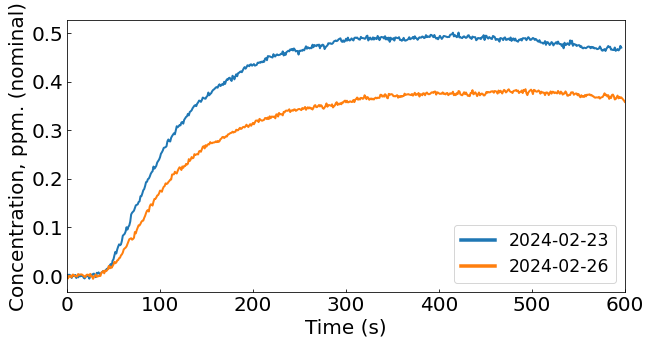
\includegraphics{figures/ch5/240223_240226_comparison_unnormalised.png}

}

}

\end{minipage}%
%
\begin{minipage}[t]{0.15\linewidth}

{\centering 

~

}

\end{minipage}%
\newline
\begin{minipage}[t]{0.11\linewidth}

{\centering 

~

}

\end{minipage}%
%
\begin{minipage}[t]{0.03\linewidth}

{\centering 

\raisebox{-\height}{

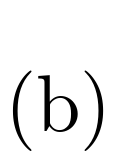
\includegraphics{figures/(b).png}

}

}

\end{minipage}%
%
\begin{minipage}[t]{0.01\linewidth}

{\centering 

~

}

\end{minipage}%
%
\begin{minipage}[t]{0.70\linewidth}

{\centering 

\raisebox{-\height}{

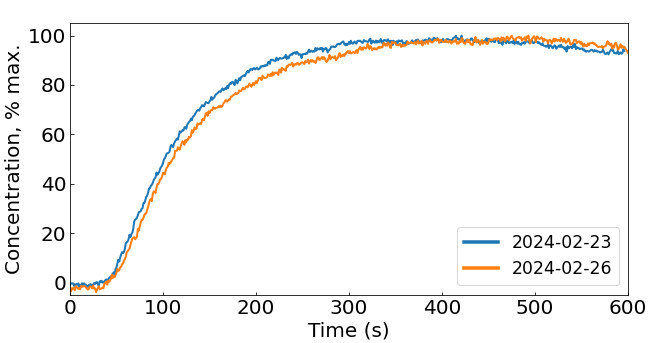
\includegraphics{figures/ch5/240223_240226_comparison.png}

}

}

\end{minipage}%
%
\begin{minipage}[t]{0.15\linewidth}

{\centering 

~

}

\end{minipage}%

\caption{\label{fig-PID-EtHex-response}The response of the
photoionisation detector to ethyl hexanoate vapour over 600 s of
exposure is shown relative to the 200 sccm nitrogen flow baseline in
(a), and normalised with respect to the maximum reading in (b).}

\end{figure}

The responses from each date are shown in
Figure~\ref{fig-PID-EtHex-response}. In
Figure~\ref{fig-PID-EtHex-response} (a), the response corresponding to
each measurement date is shown unnormalised, with the parts per million
concentration shown relative to the nitrogen baseline as recorded by the
PID. Both measurements show little to no response to vapour for
approximately 50 s, which seems to be the time taken for vapour to first
reach the PID. Over the next 100s, there is a rapid increase in vapour
concentration detected, which then settles to a constant concentration
at about 300 s. This appears to be the maximum concentration of EtHex
vapour that can be contained by the chamber in this configuration. There
is approximately a 200 parts per billion difference in maximum
concentration between the measurement on each date.

However, this is not unexpected. As discussed in
Section~\ref{sec-reference-sensors}, the PID is being run uncalibrated,
and some drift of the sensitivity of the sensor due to environmental
changes is highly likely. To check that the PID records the same
evolution of vapour flow with time, regardless of its sensitivity, the
measurements from both dates were then normalised with respect to the
maximum concentration reading. Figure~\ref{fig-PID-EtHex-response} (b)
shows that once normalised, the rate of change in concentration with
time is almost identical between the two measurement sets. This test
verifies that the evolution of vapour concentration of the device
chamber can be repeatably measured using the PID in the vapour delivery
system.

\hypertarget{photoionisation-detector-with-vapour-flow-intervals}{%
\subsubsection*{Photoionisation Detector with Vapour Flow
Intervals}\label{photoionisation-detector-with-vapour-flow-intervals}}
\addcontentsline{toc}{subsubsection}{Photoionisation Detector with
Vapour Flow Intervals}

A further series of tests were performed to verify whether it was
possible to compare different concentrations of vapour in the chamber
using the PID. All testing was performed on the same day to minimise
sensitivity drift. For each test, the system was purged of vapour and
the total dilution flow into the chamber was set at 200 sccm as read by
the Tylan mass flow controller. Flow out of the chamber to the PID was
set at 100 sccm as read by the micropump flowmeter, and the
almost-constant nitrogen baseline after 10 minutes was set as the PID
zero point. 5 mL of the volatile organic compound ethyl hexanoate
(EtHex) was placed into the analyte bottle. During each test, 200 sccm
was continuously flowed through the dilution line, except during three
evenly spaced intervals of equal length. During these intervals, 150
sccm flow was placed through the carrier line and 50 sccm flow placed
through the dilution line. In each test, the input interval time was
varied to examine its effect on maximum vapour concentration recorded by
the PID. As it took longer for the PID to return to a constant baseline
with increased input intervals, when the input interval was increased,
the spacing between intervals was also increased.

\begin{figure}

{\centering 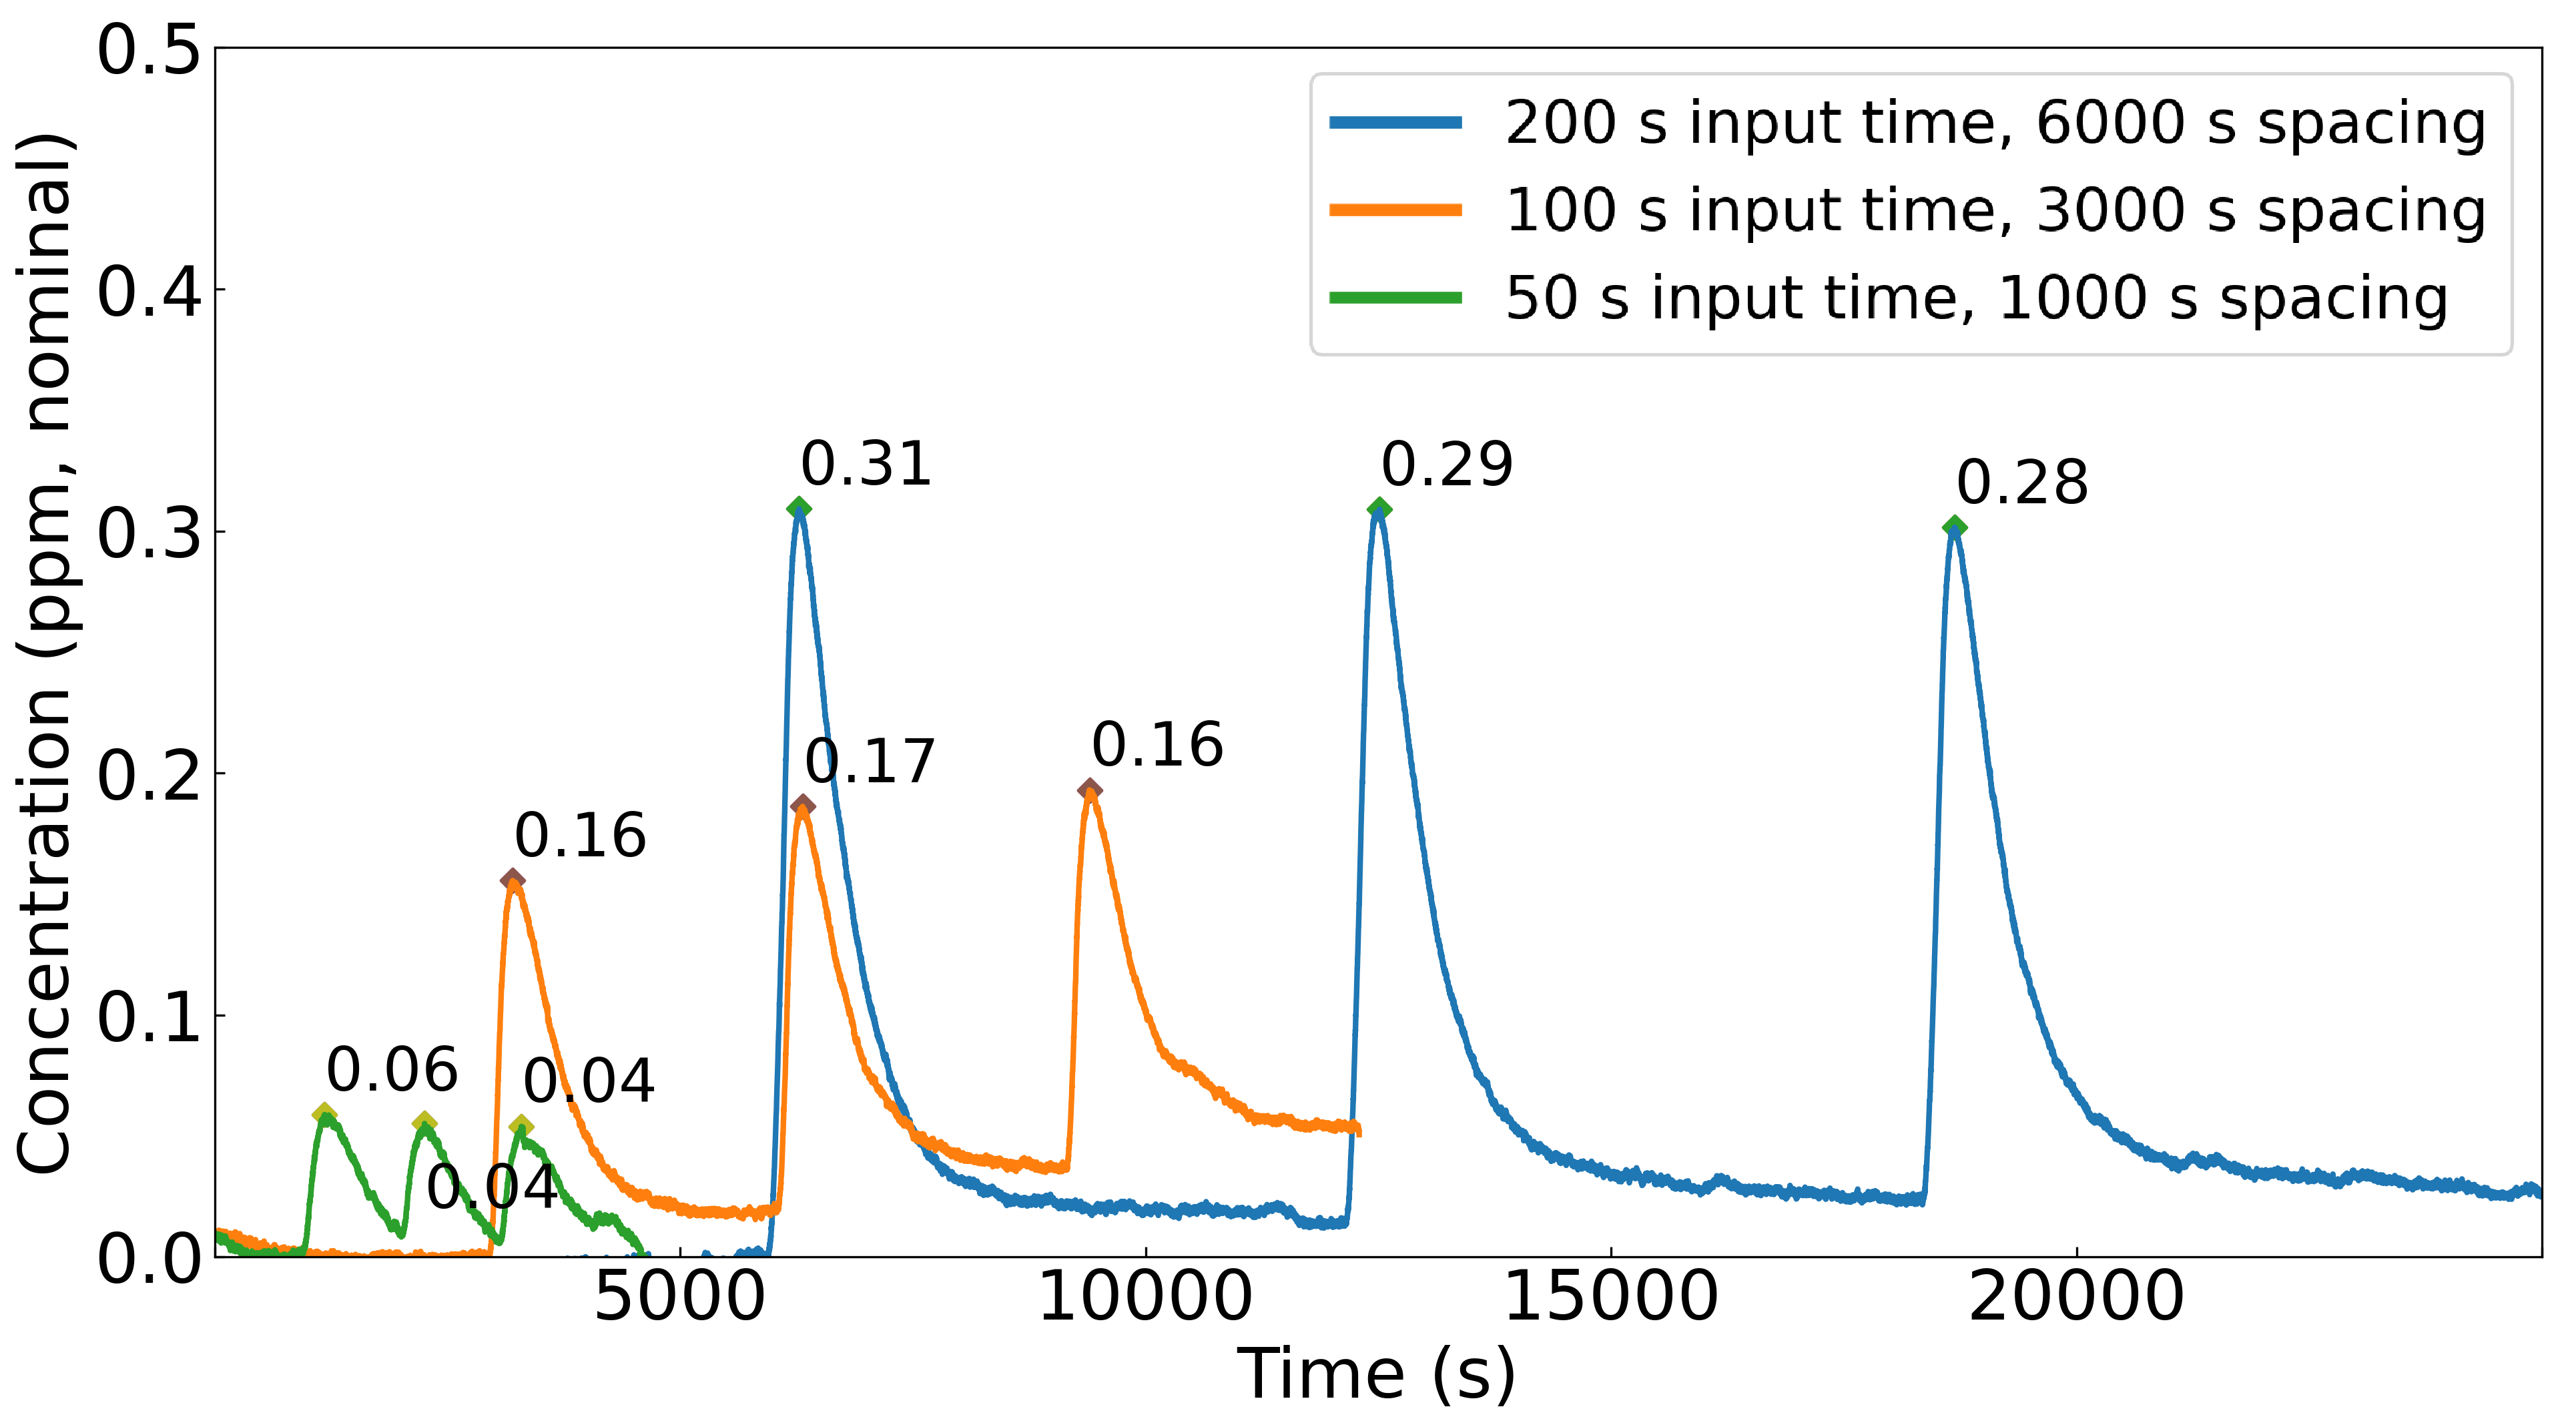
\includegraphics[width=0.7\textwidth,height=\textheight]{figures/ch5/input_time_comparison.png}

}

\caption{\label{fig-concentration-comparison}The response of the
photoionisation detector to 3 evenly-spaced intervals of ethyl hexanoate
vapour entering the device chamber, relative to a 200 sccm nitrogen flow
baseline. Input intervals were either 50 s, 100 s or 200 s in length.
During each input interval, 150 sccm carrier flow and 50 sccm dilution
flow were placed through the chamber.}

\end{figure}

The results of three tests, with input intervals of 50 s, 100 s and 200
s, are shown in Figure~\ref{fig-concentration-comparison}. Each interval
of carrier flow corresponds to a rapid increase in concentration, which
reaches a peak, then decreases. The maximum concentration reached for
each interval is shown above the corresponding peak. Note that the
maximum concentration label does not correspond to the difference
between the original baseline and the maximum concentration of each
peak. Instead, it corresponds to the difference between the
concentration measurement at a set time before the onset of carrier flow
and the maximum concentration reached. For each test, this set time is
5\% of the spacing time used, 50 s, 150 s and 300 s respectively. This
approach was taken to account for what appears to be drift from the
original 0 ppm baseline. This variable baseline drift was particularly
significant for the 100 s interval measurements, where concentration
measurements settled to a new baseline of \(\sim\) 0.05 ppm after the
third peak.

The values of the three concentration maxima in each test shown in
Figure~\ref{fig-concentration-comparison} are highly consistent, with
only a \(\pm\) 0.02 ppm margin of error. This experiment demonstrates
that if tests using the PID are performed during the same day, placing
the same vapour flow into the PID for the same interval of time in each
test, it is possible to measure the same maximum concentration with the
PID. It furthermore indicates that placing the same amount of vapour
flow into the chamber for a set amount of time leads to a reproducible
concentration of vapour building up within the chamber. Drift in the
baseline does not significantly affect the magnitude of each
concentration peak when measured relative to the baseline reading
directly before each interval.

\hypertarget{summary}{%
\section{Summary}\label{summary}}

A custom vapour delivery system was made suitable for field-effect
biosensor work through ensuring a range of flows could be delivered
through the system and that reference sensors were available for
corroboration with the readings on the field-effect biosensors. Two new
mass flow controllers with different maximum flow rates and two
reference sensors, a relative humidity and temperature sensor and
photoionisation detector, were introduced to the system in a two-stage
design process. A new electronic control system and LabView software
were designed and constructed for the altered delivery system. The
nitrogen flow through the system was then calibrated using water
displacement testing, and it was verified that the reference sensors
both worked as expected. The vapour delivery system and associated
reference sensors were tested with pristine devices in
\textbf{?@sec-pristine-characteristics}, and with insect odorant
receptor functionalised devices in \textbf{?@sec-biosensing-iORs}.

\bookmarksetup{startatroot}

\hypertarget{references}{%
\chapter*{References}\label{references}}
\addcontentsline{toc}{chapter}{References}

\markboth{References}{References}

\printbibliography[heading=none]

\cleardoublepage
\phantomsection
\addcontentsline{toc}{part}{Appendices}
\appendix

\hypertarget{vapour-system-hardware}{%
\chapter{Vapour System Hardware}\label{vapour-system-hardware}}


\hypertarget{tbl-vapour-sensor-components}{}
\begin{longtable}[t]{>{\raggedright\arraybackslash}p{5.5cm}>{\raggedright\arraybackslash}p{4.5cm}>{\raggedright\arraybackslash}p{3.75cm}}
\caption{\label{tbl-vapour-sensor-components}Major components used in construction of the vapour delivery system
described in this thesis. }\tabularnewline

\toprule
Description & Part No. & Manufacturer\\
\midrule
Mass flow controller, 20 sccm full scale & GE50A-013201SBV020 & MKS Instruments\\
Mass flow controller, 200 sccm full scale & GE50A-013202SBV020 & MKS Instruments\\
Mass flow controller, 500 sccm full scale & FC-2901V & Tylan\\
Analogue flowmeter, 240 sccm max. flow & 116261-30 & Dwyer\\
Micro diaphragm pump & P200-B3C5V-35000 & Xavitech\\
\addlinespace
Analogue flow controller, for micro diaphragm pump & X3000450 & Xavitech\\
10 mL Schott bottle & 218010802 & Duran\\
PTFE connection cap system & Z742273 & Duran\\
Baseline VOC-TRAQ flow cell, purple & 043-950 & Ametek Mocon\\
Baseline VOC-TRAQ flow cell, red & 043-951 & Ametek Mocon\\
\addlinespace
Humidity and temperature sensor & T9602-5-A & Telaire\\
Enclosure, for humidity and temperature sensor & MC001189 & Multicomp Pro\\
\bottomrule
\end{longtable}

\hypertarget{python-code-for-data-analysis}{%
\chapter{Python Code for Data
Analysis}\label{python-code-for-data-analysis}}

\hypertarget{code-repository}{%
\section{Code Repository}\label{code-repository}}

The code used for general analysis of field-effect transistor devices in
this thesis was written with Python 3.8.8. Contributors to the code used
include Erica Cassie, Erica Happe, Marissa Dierkes and Leo Browning. The
code is located on GitHub and the research group OneDrive, and is
available on request.

\hypertarget{sec-histogram-analysis}{%
\section{Atomic Force Microscope Histogram
Analysis}\label{sec-histogram-analysis}}

The purpose of this code is to analyse atomic force microscope (AFM)
images of carbon nanotube networks in .xyz format taken using an atomic
force microscope and processed in Gwyddion (see
\textbf{?@sec-afm-characterisation}). It was originally designed by
Erica Happe in Matlab, and adapted by Marissa Dierkes and myself for use
in Python. The code imports the .xyz data and sorts it into bins 0.15 nm
in size for processing. To perform skew-normal distribution fits, both
\emph{scipy.optimize.curve\_fit} and \emph{scipy.stats.skewnorm} modules
are used in this code.

\hypertarget{sec-raman-analysis}{%
\section{Raman Spectroscopy Analysis}\label{sec-raman-analysis}}

The purpose of this code is to analyse a series of Raman spectra taken
at different points on a single film (see
\textbf{?@sec-raman-characterisation}). Data is imported in a series of
tab-delimited text files, with the low wavenumber spectrum (100
cm\(^{-1} - 650\) cm\(^{-1}\)) and high wavenumber spectrum (1300
cm\(^{-1} - 1650\) cm\(^{-1}\)) imported in separate datafiles for each
scan location.

\hypertarget{sec-field-effect-transistor-analysis}{%
\section{Field-Effect Transistor
Analysis}\label{sec-field-effect-transistor-analysis}}

The purpose of this code is to analyse electrical measurements taken of
field-effect transistor (FET) devices. Electrical measurements were
either taken from the Keysight 4156C Semiconductor Parameter Analyser,
National Instruments NI-PXIe or Keysight B1500A Semiconductor Device
Analyser as discussed in \textbf{?@sec-electrical-characterisation}; the
code is able to analyse data in .csv format taken from all three
measurement setups. The main Python file in the code base consists of
three related but independent modules: the first analyses and plots
sensing data from the FET devices, the second analyses and plots
transfer characteristics from channels across a device, and the third
compares individual channel characteristics before and after a
modification or after each of several modifications. The code base also
features a separate config file and style sheet which govern the
behaviour of the main code. The code base was designed collaboratively
by myself and Erica Cassie over GitHub using the Sourcetree Git GUI.


\backmatter
\printbibliography[title=References]


\end{document}
